% Options for packages loaded elsewhere
% Options for packages loaded elsewhere
\PassOptionsToPackage{unicode}{hyperref}
\PassOptionsToPackage{hyphens}{url}
\PassOptionsToPackage{dvipsnames,svgnames,x11names}{xcolor}
%
\documentclass[
  letterpaper,
  DIV=11,
  numbers=noendperiod]{scrreprt}
\usepackage{xcolor}
\usepackage{amsmath,amssymb}
\setcounter{secnumdepth}{2}
\usepackage{iftex}
\ifPDFTeX
  \usepackage[T1]{fontenc}
  \usepackage[utf8]{inputenc}
  \usepackage{textcomp} % provide euro and other symbols
\else % if luatex or xetex
  \usepackage{unicode-math} % this also loads fontspec
  \defaultfontfeatures{Scale=MatchLowercase}
  \defaultfontfeatures[\rmfamily]{Ligatures=TeX,Scale=1}
\fi
\usepackage{lmodern}
\ifPDFTeX\else
  % xetex/luatex font selection
\fi
% Use upquote if available, for straight quotes in verbatim environments
\IfFileExists{upquote.sty}{\usepackage{upquote}}{}
\IfFileExists{microtype.sty}{% use microtype if available
  \usepackage[]{microtype}
  \UseMicrotypeSet[protrusion]{basicmath} % disable protrusion for tt fonts
}{}
\makeatletter
\@ifundefined{KOMAClassName}{% if non-KOMA class
  \IfFileExists{parskip.sty}{%
    \usepackage{parskip}
  }{% else
    \setlength{\parindent}{0pt}
    \setlength{\parskip}{6pt plus 2pt minus 1pt}}
}{% if KOMA class
  \KOMAoptions{parskip=half}}
\makeatother
% Make \paragraph and \subparagraph free-standing
\makeatletter
\ifx\paragraph\undefined\else
  \let\oldparagraph\paragraph
  \renewcommand{\paragraph}{
    \@ifstar
      \xxxParagraphStar
      \xxxParagraphNoStar
  }
  \newcommand{\xxxParagraphStar}[1]{\oldparagraph*{#1}\mbox{}}
  \newcommand{\xxxParagraphNoStar}[1]{\oldparagraph{#1}\mbox{}}
\fi
\ifx\subparagraph\undefined\else
  \let\oldsubparagraph\subparagraph
  \renewcommand{\subparagraph}{
    \@ifstar
      \xxxSubParagraphStar
      \xxxSubParagraphNoStar
  }
  \newcommand{\xxxSubParagraphStar}[1]{\oldsubparagraph*{#1}\mbox{}}
  \newcommand{\xxxSubParagraphNoStar}[1]{\oldsubparagraph{#1}\mbox{}}
\fi
\makeatother


\usepackage{longtable,booktabs,array}
\usepackage{calc} % for calculating minipage widths
% Correct order of tables after \paragraph or \subparagraph
\usepackage{etoolbox}
\makeatletter
\patchcmd\longtable{\par}{\if@noskipsec\mbox{}\fi\par}{}{}
\makeatother
% Allow footnotes in longtable head/foot
\IfFileExists{footnotehyper.sty}{\usepackage{footnotehyper}}{\usepackage{footnote}}
\makesavenoteenv{longtable}
\usepackage{graphicx}
\makeatletter
\newsavebox\pandoc@box
\newcommand*\pandocbounded[1]{% scales image to fit in text height/width
  \sbox\pandoc@box{#1}%
  \Gscale@div\@tempa{\textheight}{\dimexpr\ht\pandoc@box+\dp\pandoc@box\relax}%
  \Gscale@div\@tempb{\linewidth}{\wd\pandoc@box}%
  \ifdim\@tempb\p@<\@tempa\p@\let\@tempa\@tempb\fi% select the smaller of both
  \ifdim\@tempa\p@<\p@\scalebox{\@tempa}{\usebox\pandoc@box}%
  \else\usebox{\pandoc@box}%
  \fi%
}
% Set default figure placement to htbp
\def\fps@figure{htbp}
\makeatother


% definitions for citeproc citations
\NewDocumentCommand\citeproctext{}{}
\NewDocumentCommand\citeproc{mm}{%
  \begingroup\def\citeproctext{#2}\cite{#1}\endgroup}
\makeatletter
 % allow citations to break across lines
 \let\@cite@ofmt\@firstofone
 % avoid brackets around text for \cite:
 \def\@biblabel#1{}
 \def\@cite#1#2{{#1\if@tempswa , #2\fi}}
\makeatother
\newlength{\cslhangindent}
\setlength{\cslhangindent}{1.5em}
\newlength{\csllabelwidth}
\setlength{\csllabelwidth}{3em}
\newenvironment{CSLReferences}[2] % #1 hanging-indent, #2 entry-spacing
 {\begin{list}{}{%
  \setlength{\itemindent}{0pt}
  \setlength{\leftmargin}{0pt}
  \setlength{\parsep}{0pt}
  % turn on hanging indent if param 1 is 1
  \ifodd #1
   \setlength{\leftmargin}{\cslhangindent}
   \setlength{\itemindent}{-1\cslhangindent}
  \fi
  % set entry spacing
  \setlength{\itemsep}{#2\baselineskip}}}
 {\end{list}}
\usepackage{calc}
\newcommand{\CSLBlock}[1]{\hfill\break\parbox[t]{\linewidth}{\strut\ignorespaces#1\strut}}
\newcommand{\CSLLeftMargin}[1]{\parbox[t]{\csllabelwidth}{\strut#1\strut}}
\newcommand{\CSLRightInline}[1]{\parbox[t]{\linewidth - \csllabelwidth}{\strut#1\strut}}
\newcommand{\CSLIndent}[1]{\hspace{\cslhangindent}#1}



\setlength{\emergencystretch}{3em} % prevent overfull lines

\providecommand{\tightlist}{%
  \setlength{\itemsep}{0pt}\setlength{\parskip}{0pt}}



 


\KOMAoption{captions}{tableheading}
\usepackage{multirow}
\usepackage{pdfpages}
\makeatletter
\@ifpackageloaded{bookmark}{}{\usepackage{bookmark}}
\makeatother
\makeatletter
\@ifpackageloaded{caption}{}{\usepackage{caption}}
\AtBeginDocument{%
\ifdefined\contentsname
  \renewcommand*\contentsname{Table of contents}
\else
  \newcommand\contentsname{Table of contents}
\fi
\ifdefined\listfigurename
  \renewcommand*\listfigurename{List of Figures}
\else
  \newcommand\listfigurename{List of Figures}
\fi
\ifdefined\listtablename
  \renewcommand*\listtablename{List of Tables}
\else
  \newcommand\listtablename{List of Tables}
\fi
\ifdefined\figurename
  \renewcommand*\figurename{Figure}
\else
  \newcommand\figurename{Figure}
\fi
\ifdefined\tablename
  \renewcommand*\tablename{Table}
\else
  \newcommand\tablename{Table}
\fi
}
\@ifpackageloaded{float}{}{\usepackage{float}}
\floatstyle{ruled}
\@ifundefined{c@chapter}{\newfloat{codelisting}{h}{lop}}{\newfloat{codelisting}{h}{lop}[chapter]}
\floatname{codelisting}{Listing}
\newcommand*\listoflistings{\listof{codelisting}{List of Listings}}
\makeatother
\makeatletter
\makeatother
\makeatletter
\@ifpackageloaded{caption}{}{\usepackage{caption}}
\@ifpackageloaded{subcaption}{}{\usepackage{subcaption}}
\makeatother
\usepackage{bookmark}
\IfFileExists{xurl.sty}{\usepackage{xurl}}{} % add URL line breaks if available
\urlstyle{same}
\hypersetup{
  pdftitle={FG-COMPASS Manual},
  pdfauthor={Furtado, Ovande Jr; Jere Gallagher},
  colorlinks=true,
  linkcolor={blue},
  filecolor={Maroon},
  citecolor={Blue},
  urlcolor={Blue},
  pdfcreator={LaTeX via pandoc}}


\title{FG-COMPASS Manual}
\author{Furtado, Ovande Jr \and Jere Gallagher}
\date{2025-04-01}
\begin{document}
\maketitle

\renewcommand*\contentsname{Table of contents}
{
\hypersetup{linkcolor=}
\setcounter{tocdepth}{2}
\tableofcontents
}

\bookmarksetup{startatroot}

\chapter*{Preface}\label{preface}
\addcontentsline{toc}{chapter}{Preface}

\markboth{Preface}{Preface}

Fundamental Movement Skills (FMS) lie at the heart of children's overall
development, serving as the building blocks for a lifetime of active and
healthy living. The Furtado-Gallagher Children Observational Movement
Pattern Assessment System (FG-COMPASS) was created to provide a
user-friendly, evidence-based method for assessing these skills in
children aged 5 to 10 years. Building upon well-established theories and
previous research in motor development, this manual offers educators,
researchers, coaches, and healthcare professionals a clear framework for
understanding, administering, and interpreting the FG-COMPASS.

\section*{A Journey of Research and
Practice}\label{a-journey-of-research-and-practice}
\addcontentsline{toc}{section}{A Journey of Research and Practice}

\markright{A Journey of Research and Practice}

Over the past decade, considerable effort has been devoted to refining
the FG-COMPASS to ensure that it is practical, psychometrically sound,
and accessible to both novice and expert raters. Early work focused on
establishing expert-rater agreement and verifying the instrument's
inter- and intra-rater reliability, ensuring that FG-COMPASS scores
accurately represent a child's skill proficiency. Subsequent
investigations addressed the addition of new locomotor tasks---such as
the vertical jump and gallop---and confirmed that these expanded scales
maintained the high reliability and consistency standards set by the
original assessment. Through these enhancements, the FG-COMPASS offers a
comprehensive view of key FMS that are commonly taught and developed
across preschool and elementary-age programs.

\section*{Bridging Theory and
Practice}\label{bridging-theory-and-practice}
\addcontentsline{toc}{section}{Bridging Theory and Practice}

\markright{Bridging Theory and Practice}

While multiple FMS assessments exist, many either demand extensive
training and video review or else focus narrowly on specific tasks. By
drawing on both the composite decision-tree approach and
well-established developmental sequences, the FG-COMPASS strikes a
balance: It narrows down each skill to a few critical performance
criteria yet gives raters the information needed to classify children's
proficiency levels accurately and consistently. This streamlined design
makes it more feasible for use in real-world settings, such as physical
education classes, sports clinics, and recreational
programs---environments in `which time and resources are often limited.

\section*{Supporting All Learners}\label{supporting-all-learners}
\addcontentsline{toc}{section}{Supporting All Learners}

\markright{Supporting All Learners}

One of the central aims of this tool is to facilitate early detection of
children who may require additional support in mastering fundamental
movement skills. Research consistently links the quality of FMS to
positive outcomes in physical health, cognitive development, and
social-emotional well-being. By equipping practitioners with the means
to detect deficits early on---and to monitor progress over time---the
FG-COMPASS fosters an inclusive environment where instruction can be
tailored to each child's unique developmental trajectory.

\section*{How to Use This Manual}\label{how-to-use-this-manual}
\addcontentsline{toc}{section}{How to Use This Manual}

\markright{How to Use This Manual}

This manual is designed with clarity and practicality in mind. In the
opening chapters, readers will find an overview of core concepts in FMS
development, along with the theoretical underpinnings of the FG-COMPASS.
Subsequent sections provide step-by-step administration procedures,
including detailed rating scales, setup instructions, and scoring
guidelines for each of the ten FMS evaluated. The appendices contain
testing protocols and sample group record forms to ensure smooth
execution, whether assessments are conducted live or via video review.

\section*{Acknowledgments}\label{acknowledgments}
\addcontentsline{toc}{section}{Acknowledgments}

\markright{Acknowledgments}

The creation and refinement of the FG-COMPASS would not have been
possible without the dedication of numerous colleagues, research
assistants, and educators who contributed their time and expertise.
Their insightful feedback has helped shape an assessment tool that
balances scientific rigor with everyday utility. Special thanks go to
the children, parents, teachers, and administrators who allowed us to
pilot-test the FG-COMPASS in diverse settings, providing invaluable data
that guided ongoing improvements.

In addition to the many individuals who contributed to the development
of the FG-COMPASS, I wish to express my deepest admiration and gratitude
to my mentor and graduate advisor, Dr.~Jere D. Gallagher. Dr.~Gallagher
was a distinguished professor and associate dean at the University of
Pittsburgh's School of Education, renowned for her expertise in child
development and motor learning. She dedicated over 25 years to directing
the Kinder Kinetics Program, now known as ``Pitt's Kids: Honoring the
Vision of Dr.~Jere Gallagher,'' nationally recognized for its innovative
approach to promoting healthy movement among children aged 3 to 12.  

Dr.~Gallagher's commitment to student advocacy and inclusive education
left an indelible mark on all who had the privilege of working with her.
Her mentorship was characterized by unwavering support, insightful
guidance, and a genuine passion for fostering growth in others. She was
instrumental in shaping my academic journey, encouraging a balance of
scientific rigor and compassionate practice that continues to influence
my work today.

Her legacy endures through the many students she mentored, the programs
she established, and the lives she touched. It is with profound respect
and heartfelt appreciation that I dedicate this work to her memory. 

\textbf{Collaborative Efforts}

The FG-COMPASS is the result of collaborative efforts with many
individuals and organizations. I extend my gratitude to the following
contributors:

Dr.~Jere D. Gallagher, Oldemar Mazzardo, Fabio Fontana, Wagner de
Campos, Priscila Cacola, Lino Perez, Mackinsey Woolever, Comfort
Mokgothu, Hasan F. Mavi, Mariah Bolin, Takato Sacurai, Lawrence Ho,
Thomas Cunningham, Alan Chapla.

I also have many institutions to thank for their support, including the
University of Pittsburgh, Eastern Illinois University, California State
University - Northridge, the Western Paraná State University, and the
Paraná Federal University. Their commitment to advancing research in
motor development has been invaluable.

\section*{Concluding Remarks}\label{concluding-remarks}
\addcontentsline{toc}{section}{Concluding Remarks}

\markright{Concluding Remarks}

The FG-COMPASS is more than just an assessment tool; it is a commitment
to understanding and nurturing the fundamental movement skills that are
essential for children's growth and development. By providing a clear,
evidence-based framework for assessing these skills, we empower
educators and practitioners to make informed decisions that can
positively impact children's lives.

As we look to the future, I encourage all users of the FG-COMPASS to
embrace its potential not only as a measurement tool but also as a means
of fostering a deeper understanding of motor development. By engaging
with the assessment process, practitioners can gain insights into each
child's unique strengths and challenges, allowing for tailored
interventions that promote skill acquisition and overall well-being.

The FG-COMPASS is designed to be adaptable, allowing for its application
in various contexts, from physical education classes to clinical
settings. It is my hope that this manual will serve as a valuable
resource for practitioners seeking to enhance their understanding of
motor development and improve their assessment practices.

In presenting this manual, my hope is that it will serve as both a
resource and a catalyst, helping practitioners not only assess motor
skills more accurately but also better understand how to nurture each
child's potential. By investing in high-quality FMS assessment, we
invest in the holistic growth of children, setting them on a path toward
vibrant, active lives.

Ovande Furtado, Jr., Ph.D. April 2025

\bookmarksetup{startatroot}

\chapter{Introduction}\label{introduction}

\bookmarksetup{startatroot}

\chapter{Purpose}\label{purpose}

This manual provides users with the knowledge and skills to effectively
administer, score, and interpret the Furtado-Gallagher Children
Observational Movement Pattern Assessment System (FG-COMPASS), ensuring
its practical application and reliability in various settings.

The FG-COMPASS an observational movement pattern assessment system
designed to evaluate fundamental movement skills (FMS) in children aged
5 to 10 years. It aims to provide a more efficient and practical
alternative to existing FMS assessment tools, such as the Test of Gross
Motor Development-2 (TGMD-2), which is widely considered the ``gold
standard'' in this area. The FG-COMPASS was developed by combining
aspects of the composite 3-stage approach and the observational plan
approach to provide a practical and efficient way for practitioners to
assess FMS in various settings.

\bookmarksetup{startatroot}

\chapter{Overview of the FG-COMPASS}\label{overview-of-the-fg-compass}

The FG-COMPASS is an observational assessment tool developed to evaluate
fundamental movement skill (FMS) development in children 5 to 10 years
old (Furtado \& Gallagher, 2018). It was developed by combining aspects
of the composite 3-stage approach (Gallahue \& Ozmun, 2002) and the
observational plan approach (Haywood \& Getchell, 2019) to provide a
practical and efficient way for practitioners to assess FMS in various
settings (Furtado \& Gallagher, 2012).

The FG-COMPASS assesses ten FMS, divided into two subtests: a locomotor
subtest with five skills (skipping, hopping, horizontal jumping,
vertical jumping, and galloping) and an object manipulation subtest with
five skills (batting, stationary dribbling, kicking, throwing, and
catching). Unlike other FMS assessment tools that use multiple
performance criteria for each skill, the instrument relies on only three
key performance criteria selected from validated and hypothesized
developmental sequences (Furtado \& Gallagher, 2018). This allows for
quicker and more practical testing administration compared to more
complex assessment instruments(Perez, 2024).

The instrument uses a process-oriented, criterion-referenced design,
focusing on the quality of movement rather than quantitative
measures(Perez, 2024). It employs a composite decision tree approach
(see Appendix A), where users make sequential decisions based on the
presence or absence of specific performance criteria to classify
children into levels 1 through 4. This approach aims to simplify the
assessment process while providing valuable information about a child's
FMS development, which can be used to evaluate the effectiveness of
instructional programs and monitor/detect deficits in FMS
development(Perez, 2024).

\section{Rating Scales}\label{rating-scales}

The FG-COMPASS was developed using a Composite Decision Tree approach
(see Figure~\ref{fig-cdt}), which combines elements of the Observational
Plan (OP)(Haywood \& Getchell, 2019) and the Three-Stage (TS)
(McClenaghan \& Gallahue, 1978)models for FMS assessment (Furtado,
2009). The word composite refers to the practice of assessing FMS as a
whole, rather than by body parts (i.e., arms, legs, torso, etc.). Even
though individual body parts are considered with the composite method,
the final score denotes proficiency levels for the entire body.

The OP model is a method for assessing motor skill development,
particularly in FMS, by systematically observing and recording movement
patterns. It emphasizes the importance of a detailed and methodical
process to ensure accuracy and reliability of observations. The TS model
is a framework for understanding motor skill development, emphasizing
the progression from initial attempts at a skill to mature execution. It
limits the classification of skills to three stages (initial,
elementary, and mature) and selects only key performance criteria for
the assessment tasks (Furtado \& Gallagher, 2012). An example of a
performance criteria assessed in the FG-COMPASS is the ``follow
through'' when kicking a stationary ball.

The composite decision trees (CDTs) for each assessment task in the
FG-COMPASS is presented in a decision-tree format to facilitate
assessment. Each CDT has three stage levels: a discriminatory-decision
level (DDL), a confirmatory-decision level (CDL), and an
outcome-decision level (ODL).

The DDL has a single decision node which comprises of one key
performance criterion that is intended to discriminate between levels 1
and 4. The CDL is comprised of two performance criteria, each with the
intention to confirm whether a performer is level 1 (if NO was selected
in the DDL) or level 4 (if YES was selected in DDL). In the case of
failing to confirm levels 1 and 4, they default to levels 2 and 3,
respectively.

\begin{figure}

\hfill\pandocbounded{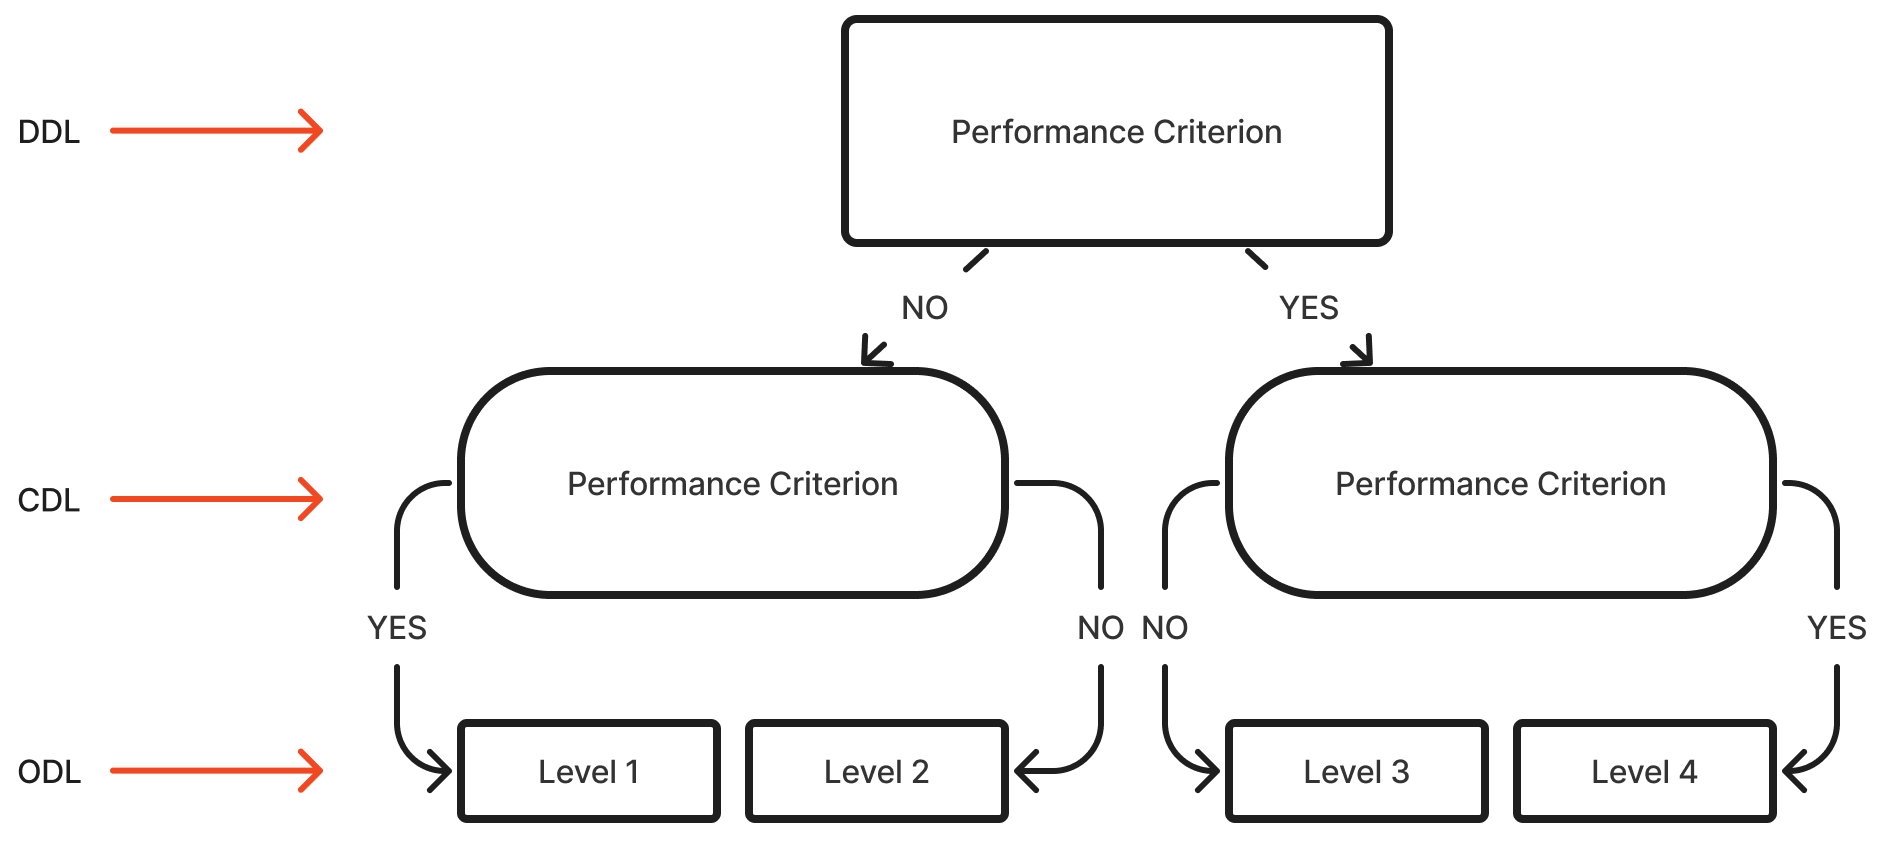
\includegraphics[keepaspectratio]{static/images/fgcompass-dt-model-stages.png}}

\caption{\label{fig-cdt}Framework model for the decision trees of the
FG-COMPASS}

\end{figure}%

The discriminatory-decision level holds a single decision-node that
contains a performance criterion that strongly discriminates between
levels 1 and 4 (Furtado \& Gallagher, 2012). The confirmatory-decision
level holds two decision-nodes that confirm the child's skill level. The
right-side confirmatory-decision node confirms the whether the child is
at level 4, while the left confirmatory-decision node is used to confirm
a level 1 skill proficiency. The outcome-decision level provides the
final classification of the child's skill level, from 1 (least
proficient) to 4 (most proficient).

By using this composite decision-tree approach, the FG-COMPASS aims to
provide a more practical approach for assessing FMS development; thus,
bypassing the need to videotape skill performance. This because it
limits the number of performance criteria and classification stages
compared to other FMS assessment tools (Furtado \& Gallagher, 2012).

\section{The Importance of Fundamental Movement Skill
Development}\label{the-importance-of-fundamental-movement-skill-development}

Fundamental movement skill development in children is pivotal to their
comprehensive growth and overall well-being. FMS encompasses fundamental
motor activities such as running, jumping, and throwing, which engage
the large muscle groups of the body. These skills are crucial for
physical, cognitive, and social development.

\subsection{Physical Activity and
Health}\label{physical-activity-and-health}

Multiple studies show positive links between FMS proficiency and
physical activity (PA) in children aged 3-10. For instance, DuBose et
al. (2018) found children engaged in more moderate to vigorous PA scored
higher in motor skills on the MABC-2. Additionally, Giuriato et al.
(2022) noted that increased lean body mass predicts gross motor
coordination (GMC), suggesting GMC development boosts healthy body
composition. Balakrishnan \& Ramalingam (2023) reported a correlation
between sensory processing abilities and gross motor skills in ages
7-10, indicating improvement in motor skills may enhance sensory
processing and physical activity engagement. FMS and PA relationship is
reciprocal, as PA aids motor skill development. Fu et al. (2022)'s
12-week functional training program showed improved GMC, fitness, and
sensory integration in healthy Chinese children aged 5--6, indicating
that targeted interventions positively impact overall fitness. Ma \& Luo
(2023) found a strong association between physical activity and both
locomotor and object control skills in preschoolers. This suggests
promoting physical activity enhances various gross motor skills,
fostering a positive cycle for children's health. Overall, these studies
indicate that FMS are vital in influencing PA levels and health in
children aged 3-10. The reciprocal relationship emphasizes the need to
promote both FMS development and PA in early childhood to foster healthy
habits and overall well-being.

\subsection{Cognitive development}\label{cognitive-development}

Numerous studies indicate substantial positive links between gross motor
skills and cognitive development in children. For example, Veldman et
al. (2019) found a connection in Australian toddlers, while Zuccarini et
al. (2020) noted cascading effects from early motor skills on later
cognitive abilities. This implies that gross motor proficiency may
influence cognitive outcomes during early childhood transition.
Additionally, research connects gross motor abilities with cognitive
domains in children aged 3-10. Fathirezaie et al. (2022) found
significant ties between executive functions, like inhibition and
working memory, and gross motor skills in rural children ages 8-10. This
suggests that better motor skills may enhance executive functions
critical for academic success. Similarly, Geertsen et al. (2016) showed
that both fine and gross motor skills correlate positively with
cognitive functions and academic performance in preadolescents,
emphasizing the importance of motor skill development for cognitive and
educational outcomes. Moreover, studies have investigated factors
affecting the motor-cognitive relationship in children aged 3-10. Viegas
et al. (2021) discovered that preschoolers with low physical activity
and cognitive function, especially girls, would likely have delayed
gross motor skills. They concluded that these factors independently
predict skill delays, indicating a direct link between motor skills and
cognitive development.

The bidirectional influence of motor and cognitive skills in children
aged 3-10 is significant; gross motor skills affect cognitive
development, and cognitive abilities facilitate motor skill acquisition.
Capio et al. (2022) established that in 5.84-year-old children, object
control skills and verbal working memory are linked, illustrating the
intricate relationship between physical, motor, and cognitive growth.
Additionally, Bedford et al. (2015) found that early gross motor skills
forecast language development in children with autism, suggesting that
motor proficiency impacts other developmental areas like language
acquisition. In conclusion, research strongly indicates that gross motor
skill proficiency is vital for cognitive development across domains in
children aged 3-10. Promoting motor skill development may yield
extensive benefits for holistic development and academic readiness
during early and middle childhood.

\subsection{Social development}\label{social-development}

Studies show a positive link between gross motor skills and social
development in children aged 3-10. Šalaj \& Masnjak (2022) found a weak
correlation between motor skills and social-emotional functioning in
preschoolers, underscoring the importance of gross motor skill
development in enhancing children's social and emotional growth. Gross
motor skills also significantly affect children's emotional
understanding and social interactions. Zhang et al. (2023) discovered
that object control skills predict emotional comprehension in ages 3-6,
suggesting that improving these skills aids in interpreting emotions
vital for social engagement. This study highlights the
interconnectedness of motor, cognitive, and socio-emotional development
in early childhood. Moreover, gross motor skills influence peer
interactions and social competence. Redondo-Tebar et al. (2021) noted
that higher motor competence is associated with better health-related
quality of life, especially in self-esteem and friendships among
typically developing children. Enhanced motor skills foster more
positive social experiences and confidence in interactions. Furthermore,
Crane et al. (2023) studied motor competence in 8-year-olds, revealing a
complex relationship between motor skills and social factors.

Lastly, the relationship between gross motor skills and social
development varies with age and other influences. Peyre et al. (2019)
found that cognitive factors predict changes in motor skills from ages 3
to 6, indicating a reciprocal relationship that can impact social
growth. Barnett et al. (2016) identified age, gender, and activity
levels as significant influences on gross motor competence. These
findings call for a broad perspective in examining how motor skills
interplay with social development.

In conclusion, the relationship between gross motor skills and social
development in 3-10-year-olds is complex and changes over time. Research
indicates that improving gross motor skills positively affects emotional
understanding, peer interactions, and overall competence. However, this
relationship varies due to multiple factors, highlighting the need for
comprehensive support in child development.

\section{Uses of the FG-COMPASS}\label{uses-of-the-fg-compass}

\subsection{Evaluating the effectiveness of instructional
programs}\label{evaluating-the-effectiveness-of-instructional-programs}

Evaluating the effectiveness of instructional programs aimed at
improving children's movement skills is a critical application of the
FG-COMPASS. By using this tool to assess student outcomes before and
after implementing new educational initiatives, professionals can
determine whether their interventions are having a positive impact on
student skill learning. This information enables teachers to refine
their instruction, make adjustments as needed, and ultimately improve
the overall quality of education provided to their students.
Furthermore, evaluating program effectiveness also allows educators to
share best practices with colleagues, promoting a culture of
collaboration and continuous improvement within schools.

\subsection{Monitoring and Detecting
Deficits}\label{monitoring-and-detecting-deficits}

Monitoring the longitudinal development of students' FMS is essential in
educational settings, enabling professionals to systematically track
progress and make evidence-based decisions regarding instructional
strategies. Regular assessment of FMS allows practitioners to identify
specific areas where children may require additional support or
demonstrate mastery in FMS, facilitating the customization of teaching
methods to address each student's distinct developmental needs.
Additionally, detecting deficits in FMS development allows professionals
to provide targeted interventions, helping students catch up and
overcome challenges. Early identification enables teachers to modify
their instruction, making it more inclusive and accessible, thereby
contributing to a more positive and supportive learning environment
where every child feels valued and encouraged to succeed.

\bookmarksetup{startatroot}

\chapter{Content Validity}\label{content-validity}

To establish the content validity of the FG-COMPASS, we undertook a
systematic evaluation process led by experts. This approach combined
quantitative ratings with valuable qualitative feedback (Furtado, 2004).
We began by selecting a panel of 20 content experts, which included
eight university professors and twelve experienced physical education
teachers. Their extensive theoretical knowledge and practical experience
made them well-equipped to provide insightful judgments. We initiated
contact with these experts using a standardized protocol, starting with
phone calls followed by detailed email instructions to ensure clarity.

We created an Internet-based item review form to gather evidence at both
the item and test levels. Experts were asked to evaluate each proposed
test item---targeting both movement concepts and fundamental movement
skills---using a 4-point Likert scale that ranged from ``not important
at all'' to ``very important.'' Additionally, a 5-point scale was
employed at the test level to assess how well the item pool aligned with
the overall purpose of the test and its representativeness in relation
to content taught in physical education. This dual approach allowed us
to thoroughly scrutinize both individual components and the integrated
set of items.

When it came to data analysis, we employed both quantitative and
qualitative methods. We calculated descriptive statistics, such as
percentage distributions and median scores, to see if the items met our
acceptance criteria---specifically, we set a threshold that required at
least 67\% of respondents to rate an item as ``very'' or ``moderately''
important. Alongside this, we carefully analyzed the qualitative
comments from the experts to identify items that might have been overly
specific, too easy, or not aligned with the intended domain. This
careful and comprehensive analysis guided our decisions on whether to
revise, collapse, or exclude certain items.

In the end, this iterative refinement process enabled us to adjust the
initial pool of 31 items based on the expert input we received. The
combination of expert feedback and statistical analysis ensured that the
final test content accurately represented the domains of movement
concepts and fundamental movement skills as defined in the National
Standards for Physical Education. This thorough process not only
provided strong initial support for the content-related validity of our
assessment tool but also highlighted its relevance for tracking
individual progress, evaluating instructional effectiveness, and
pinpointing specific deficits in motor skill development.

\bookmarksetup{startatroot}

\chapter{Expert-Rater Agreement}\label{expert-rater-agreement}

Expert-rater agreement is a crucial aspect of establishing the
reliability and validity of any assessment tool, including the
FG-COMPASS. In the context of the FG-COMPASS, expert-rater agreement
refers to the level of consistency and agreement among trained raters
when scoring children's performance on the assessment tasks. This is
particularly important because the FG-COMPASS relies on observational
assessments, which can be subjective and influenced by individual
raters' interpretations.

The evolution of the FG‑COMPASS has been marked by continuous efforts to
enhance its reliability and utility as an observational tool for
assessing fundamental movement skills in children. Early work by Furtado
\& Gallagher (2012) laid the foundation by demonstrating acceptable
expert‑rater agreement on the original set of 11 rating scales, with
weighted kappa values ranging from 0.51 to 0.85 (mean = 0.71). These
findings established a solid basis for the instrument's reliability and
led to targeted refinements in subsequent research.

In their follow‑up investigation, Furtado \& Gallagher (2018) revisited
and modified the original scales, resulting in improved agreement for
most measures. Their study confirmed that four of the revised scales
achieved ``good'' to ``very good'' expert‑rater agreement. In contrast,
the scales for side sliding and leaping---due to persistent subjectivity
and inconsistency---were removed from the test.

Building on this extensive groundwork, Perez (2024) extended the
instrument by investigating the inclusion of two new locomotor
skills---vertical jump and gallop---to further improve the FG‑COMPASS.
In their study, 60 children aged 5--10 years were filmed performing
these new skills, and an expert used newly developed rating scales,
based on literature‑supported performance criteria, to classify the
performances. Thirty undergraduate raters underwent comprehensive
training and then rated a set of video clips. The expert‑non‑expert
agreement for the new vertical jump scale was exceptionally high
(weighted kappa = 0.96, ICC = 0.98), while the gallop scale also
demonstrated strong agreement (weighted kappa = 0.89, ICC = 0.94).
Inter‑rater reliability among non‑expert raters was very good for
vertical jump (mean kappa = 0.92) and reached a moderate level for
gallop (mean kappa = 0.78), with intra‑rater reliability similarly
robust for both skills.

Collectively, the findings of these studies indicate that the FG‑COMPASS
can be relied upon for consistent classification decisions. The initial
work by Furtado and Gallagher (2012, 2018) established strong
expert‑rater agreement and consistency across the original skills, and
the subsequent inclusion of vertical jump and gallop, as investigated by
Perez and Furtado (2024), expands the scope of the locomotor subscale
without compromising the instrument's reliability. This progression
underscores the FG‑COMPASS's potential as a practical and objective tool
for assessing FMS development in children, supporting its adoption in
both research and educational contexts.

\bookmarksetup{startatroot}

\chapter{Inter-Rater Reliability}\label{inter-rater-reliability}

Inter‑rater reliability for the FG‑COMPASS has been examined and
re‑examined through multiple studies. In the initial work by Furtado \&
Gallagher (2012), raters, who received standardized training,
independently coded videotaped fundamental movement skills. Weighted
kappa analyses revealed agreement values ranging from 0.51 to 0.85
(mean\,=\,0.71), establishing an already ``good'' level of inter‑rater
consistency for the original set of rating scales.

Finally, Woolever (2016) investigated live assessments (as opposed to
video‑based ones) and found that inter‑rater reliability remained
``good,'' albeit somewhat lower than the strong values observed under
controlled video conditions. Even so, their results supported the
FG‑COMPASS as a practical tool for real‑world educational or research
settings, where live evaluations are often needed.

A subsequent refinement by Furtado \& Gallagher (2018) involved slight
revisions to the locomotor domain. Once again, multiple raters underwent
systematic training and then independently scored children's recorded
performances. Here, the combined locomotor and manipulative subtests
yielded an intraclass correlation coefficient (ICC) approaching 0.89,
indicating improved rater consensus following the scale modifications.

More recently, Perez (2024) introduced two new locomotor
skills---vertical jump and gallop---to the FG‑COMPASS. A cohort of
non‑expert raters was trained on these novel scales and asked to
evaluate videotaped performances. The vertical jump scale demonstrated
notably high inter‑rater reliability (mean weighted kappa\,=\,0.92;
ICC\,=\,0.98), while the gallop scale, though slightly lower, still
achieved robust agreement (mean weighted kappa\,=\,0.78; ICC\,=\,0.95).

Taken together, these studies consistently confirm that trained raters
can achieve sound inter‑rater reliability when using the FG‑COMPASS to
assess a broad spectrum of FMS in children, whether under controlled
video conditions or in live evaluations.

\bookmarksetup{startatroot}

\chapter{Intra-Rater Reliability}\label{intra-rater-reliability}

Intra‑rater reliability for the FG‑COMPASS has been documented in
multiple studies using a retest or repeated‑rating format, wherein the
same raters evaluated children's performances on two different occasions
and their initial and follow‑up ratings were compared. In Woolever
(2016), raters used the FG‑COMPASS in live physical education settings
and then repeated their evaluations after a short delay. Weighted kappa
statistics across locomotor and manipulative tasks ranged from about
0.70 to 0.85, indicative of ``good'' or ``excellent'' reproducibility
for individual raters under real‑world conditions.

Similarly, Furtado \& Gallagher (2018) employed a video‑based approach
in which raters first scored children's recorded performances and then
returned after an interval of approximately one week to re‑score the
same video clips in a randomized order. Both weighted kappa and
intraclass correlation coefficient (ICC) analyses confirmed ``good'' to
``excellent'' agreement between the two rounds of scoring, typically
yielding kappa values above 0.80 and ICCs near or exceeding 0.90 for
both locomotor and manipulative components.

More recently, Perez (2024) introduced two new FG‑COMPASS scales for
vertical jump and gallop and tested intra‑rater reliability in a similar
fashion. After rating a set of videos, the same raters returned one week
later to re‑score the same clips, with the mean weighted kappa for
vertical jump reaching 0.96 (ICC = 0.98), while gallop obtained 0.85
(ICC = 0.92). Taken together, these findings indicate that once raters
have received consistent FG‑COMPASS training, they can reliably
replicate their own scoring decisions over time, whether the tool is
used in controlled video reviews or during live assessments.

\bookmarksetup{startatroot}

\chapter{Concurrent Validity}\label{concurrent-validity}

Concurrent validity is a crucial aspect of establishing the
trustworthiness and practical utility of any assessment tool, especially
in the field of motor skill development. In assessing fundamental motor
skills in children, concurrent validity is particularly important
because it ensures that a new assessment tool accurately reflects the
child's actual motor abilities, aligning with established benchmarks.

In their study, Woolever (2016) investigated the instrument's concurrent
validity by comparing its results to those of the Test of Gross Motor
Development--Second Edition (TGMD‑2) (Ulrich, 2000). After children's
live skill performances were independently assessed with both tools, the
researchers used the intraclass correlation coefficient (ICC) and
Bland‑Altman analysis to evaluate the agreement between their locomotor,
manipulative, and total scores.

They found that, for the locomotor subtest (LFMS), the FG‑COMPASS and
the TGMD‑2 demonstrated an ICC of 0.68---considered ``good''
agreement---while the manipulative subtest (MFMS) reached an ICC of
0.89, classified as ``excellent.'' When combining both subtests into a
single total FMS score (TFMS), the ICC remained ``excellent'' at 0.89.
Bland‑Altman plots revealed mean biases close to zero for all three
categories, indicating minimal systematic differences between the two
assessments. Therefore, the FG‑COMPASS and the TGMD‑2 measure children's
gross motor proficiency in a sufficiently similar manner, thus
confirming the FG‑COMPASS's concurrent validity under live conditions

\bookmarksetup{startatroot}

\chapter{Procedures}\label{procedures}

\bookmarksetup{startatroot}

\chapter{Introduction}\label{introduction-1}

This section includes the Examiner Group Record Forms used to collect
FG-COMPASS data. Although performances may be videotaped for subsequent
assessment, the FG‑COMPASS was developed for live, in situ skill
performance evaluation. Test administrators must thoroughly familiarize
themselves with the testing protocols before conducting assessments.
Currently, only the paper-and-pencil version of the test is available;
however, a mobile version will be released shortly.

\bookmarksetup{startatroot}

\chapter{General Instructions}\label{general-instructions}

\begin{enumerate}
\def\labelenumi{\arabic{enumi}.}
\tightlist
\item
  Review the questions within the decision tree, ensuring they are
  consistent with the corresponding illustrations.
\item
  To promote reliable assessment, evaluate each performer across three
  trials. The behavior observed should be evident in at least two of the
  three trials to confirm consistency.
\item
  Avoid inferring performance levels based on the performer's apparent
  age, as chronological age is not indicative of optimal performance.
\item
  During demonstrations, avoid simultaneous speaking and demonstrating.
  Refrain from providing additional verbal information before or after
  the demonstration unless specifically prompted (refer to Notes for
  Examiners), as excessive information may confuse the performer.
\item
  To improve efficiency, assess three to five children simultaneously.
  Confirm that each child can view your demonstration and is following
  the instructions. In this context, demonstrations should be performed
  only once.
\end{enumerate}

\bookmarksetup{startatroot}

\chapter{Equipment}\label{equipment}

\begin{itemize}
\tightlist
\item
  4-inch balls are used for the overhand throw.
\item
  8-inch balls are used for the catch and kick.
\item
  Small and medium-sized basketballs
\item
  Nerf softballs
\item
  Floor tape
\item
  4- to 5-inch beanbags
\item
  Plastic cones
\item
  Plastic basket
\item
  Name tags
\item
  Stopwatch
\end{itemize}

\bookmarksetup{startatroot}

\chapter{Manipulative Subscale}\label{manipulative-subscale}

\section{Overhand Throw}\label{overhand-throw}

\subsection{Equipment}\label{equipment-1}

\begin{itemize}
\tightlist
\item
  Beanbags
\item
  Basket
\item
  Floor tape
\end{itemize}

\subsection{Setup}\label{setup}

\begin{itemize}
\tightlist
\item
  Tape a line 20 feet from the wall on the floor.
\item
  Stand about 10 feet from the examinee to get a side view of the
  action.
\item
  Place a bucket containing several bean bags three feet ahead of the
  line.
\end{itemize}

\subsection{Directions for performers}\label{directions-for-performers}

\begin{itemize}
\tightlist
\item
  I want to see your throw;
\item
  Walk up to the bucket, grab one beanbag, and throw it as hard as you
  can against the wall without stepping over the line;
\item
  Then do it three more times;
\item
  Watch as I demonstrate.
\end{itemize}

\subsection{Notes for examiners}\label{notes-for-examiners}

\begin{itemize}
\tightlist
\item
  Give the performer four trials (the first trial is for practice only).
\item
  Do not allow performers to step over the line.
\end{itemize}

\subsection{Scale}\label{scale}

\begin{figure}

\centering{

\pandocbounded{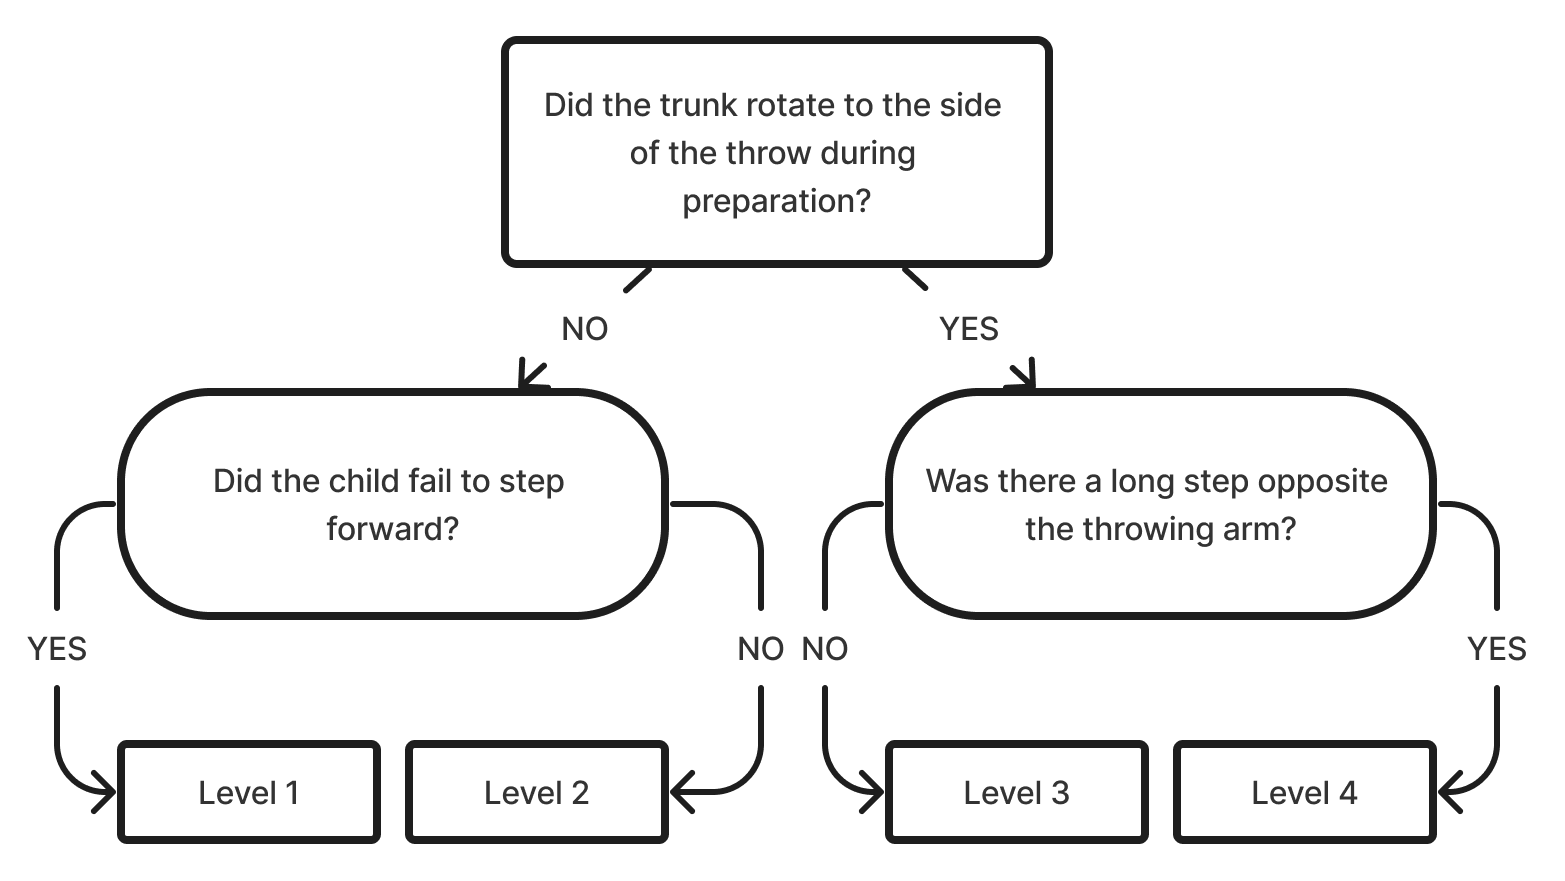
\includegraphics[keepaspectratio]{static/images/man-ot/scale-man-ot.png}}

}

\caption{\label{fig-scale-ot}Scale for Overhand Throw}

\end{figure}%

\subsection{Developmental Sequences}\label{developmental-sequences}

\begin{longtable}[]{@{}
  >{\raggedright\arraybackslash}p{(\linewidth - 2\tabcolsep) * \real{0.3500}}
  >{\raggedright\arraybackslash}p{(\linewidth - 2\tabcolsep) * \real{0.6500}}@{}}
\toprule\noalign{}
\begin{minipage}[b]{\linewidth}\raggedright
Image
\end{minipage} & \begin{minipage}[b]{\linewidth}\raggedright
Description
\end{minipage} \\
\midrule\noalign{}
\endhead
\bottomrule\noalign{}
\endlastfoot
\pandocbounded{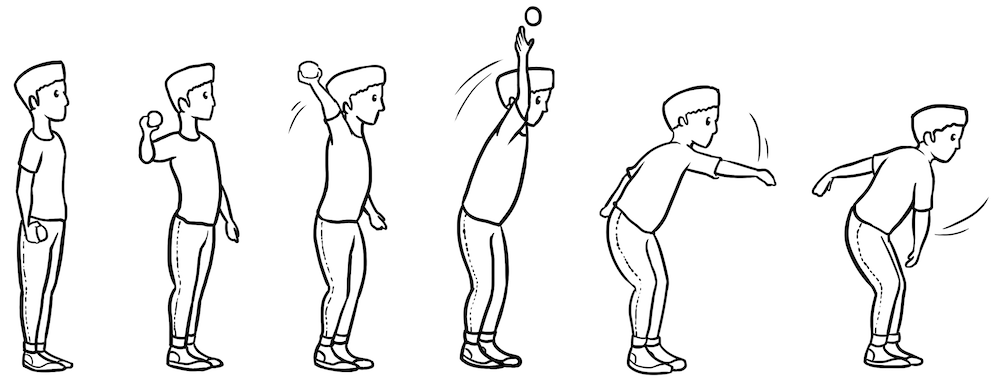
\includegraphics[keepaspectratio]{static/images/man-ot/ot1.png}}
& \textbf{Level 1}The trunk faces the target, and there is no step
forward. Jumping up and down is not considered a step forward. \\
\pandocbounded{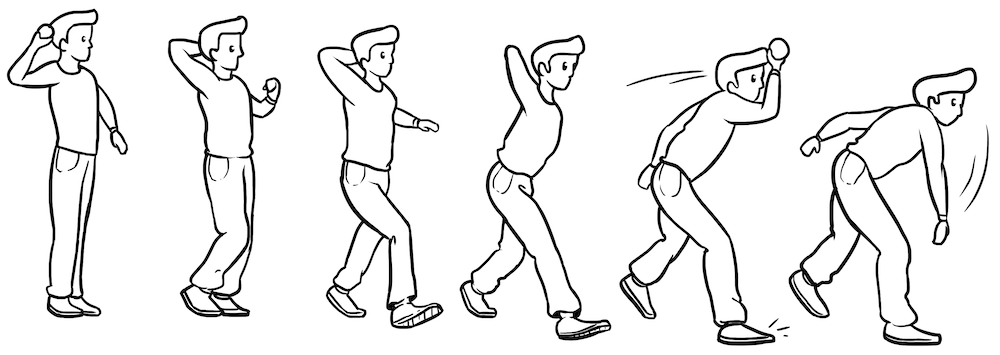
\includegraphics[keepaspectratio]{static/images/man-ot/ot2.png}}
& \textbf{Level 2}Minimal or no trunk rotation is observed during the
preparatory phase. However, a forward step is taken, using either
foot. \\
\pandocbounded{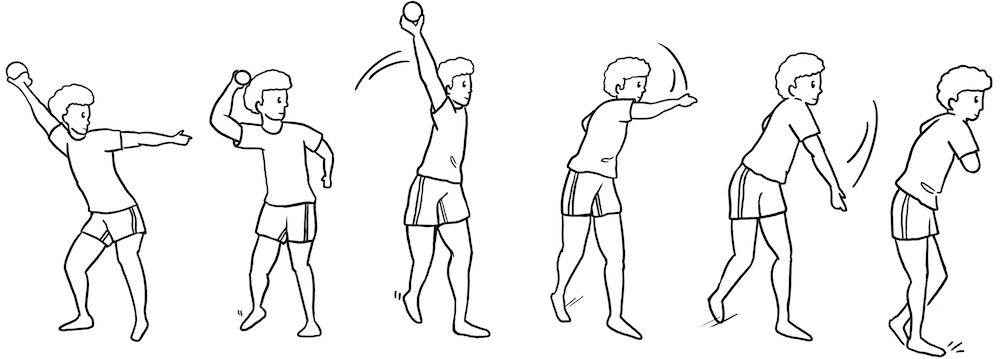
\includegraphics[keepaspectratio]{static/images/man-ot/ot3.png}}
& \textbf{Level 3}The movement involves a trunk rotation to one side and
a slight step forward with the opposite leg. \\
\pandocbounded{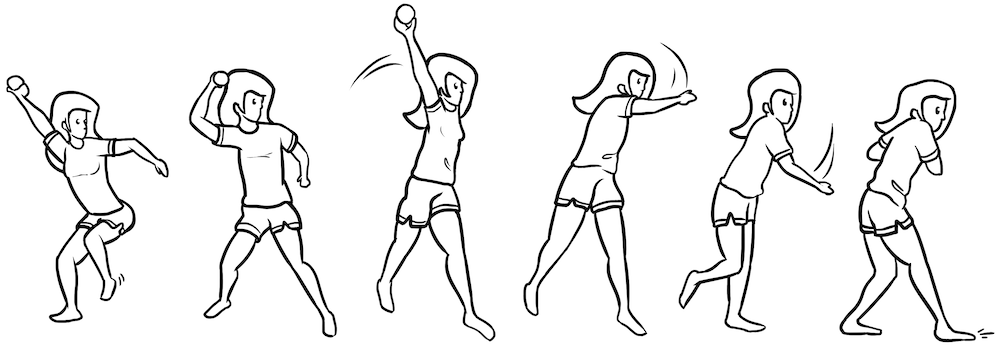
\includegraphics[keepaspectratio]{static/images/man-ot/ot4.png}}
& \textbf{Level 4}The trunk rotates to the side with a long
contralateral step forward (at least half the performer's height). \\
\end{longtable}

\section{Kick}\label{kick}

\subsection{Equipment}\label{equipment-2}

\begin{itemize}
\tightlist
\item
  8-inch balls
\item
  Floor tape
\item
  Basket
\end{itemize}

\subsection{Setup}\label{setup-1}

\begin{itemize}
\tightlist
\item
  Tape a line on the floor 20 feet from the wall (kicking line).
\item
  Stand about 10 feet from the examinee for a side view of the action.
\item
  Have a bucket with several soccer balls inside, placed 3 feet before
  the kicking line.
\end{itemize}

\subsection{Directions for
performers}\label{directions-for-performers-1}

\begin{itemize}
\tightlist
\item
  I want to see your kick.
\item
  Walk up to the bucket, grab a soccer ball, place it on the kicking
  line, and then kick it against the wall.
\item
  Then, repeat it three more times.
\item
  Watch as I demonstrate.
\end{itemize}

\subsection{Notes for examiners}\label{notes-for-examiners-1}

\begin{itemize}
\tightlist
\item
  Give the performer four trials (the first trial is for practice only).
\item
  Sometimes a child runs towards the ball, stops, and then kicks it.
  This is the same as not taking any steps toward the ball.
\item
  Swinging the body back and forward before the kick is not a complete
  step.
\end{itemize}

\subsection{Scale}\label{scale-1}

\begin{figure}

\centering{

\pandocbounded{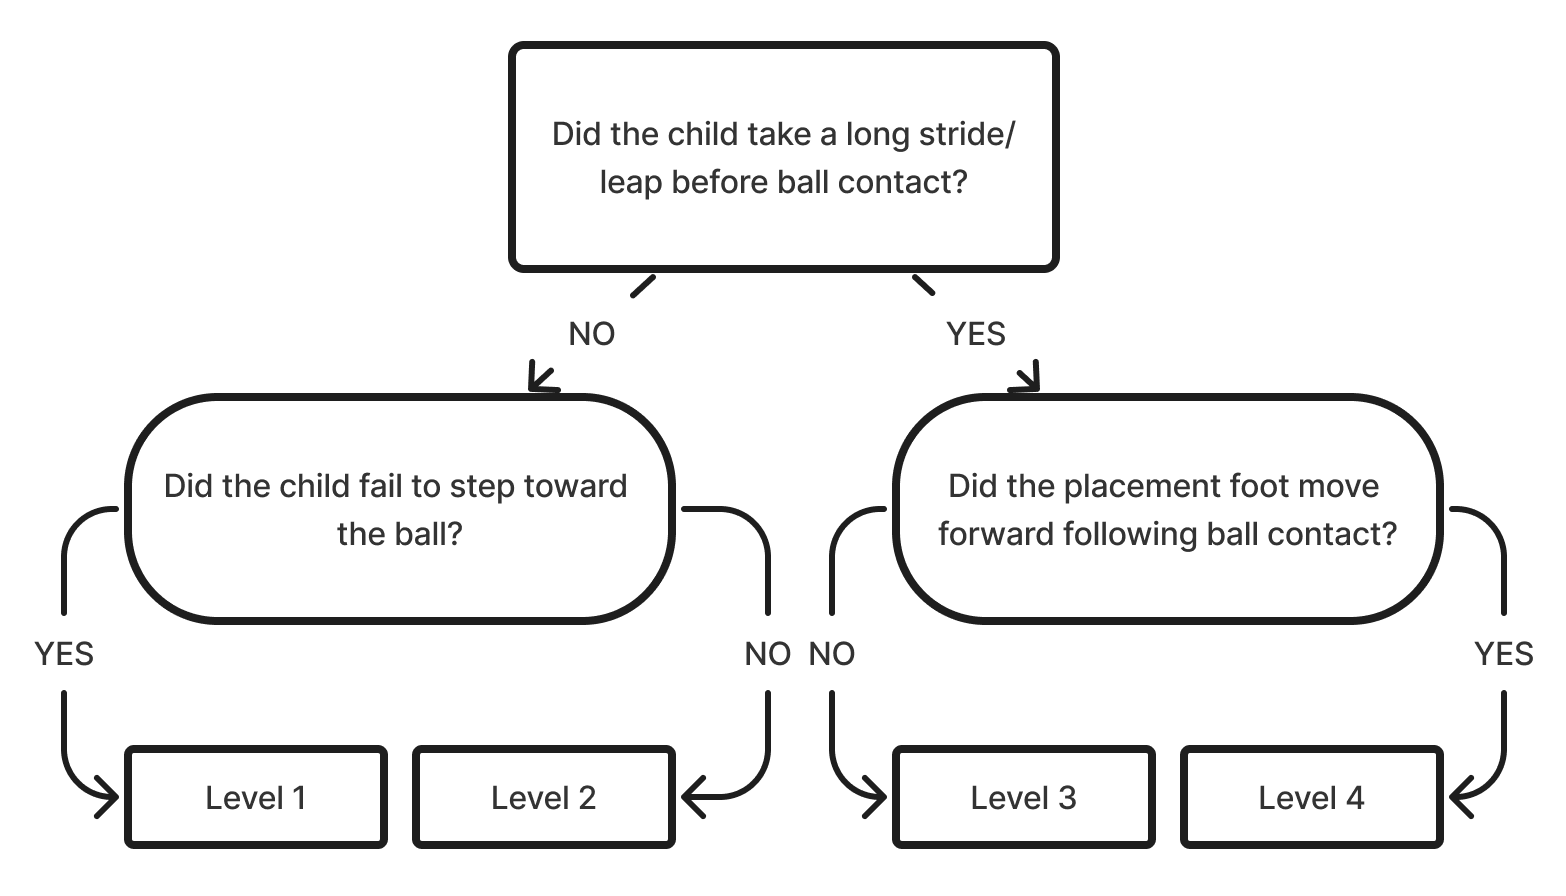
\includegraphics[keepaspectratio]{static/images/man-kick/scale-man-kick.png}}

}

\caption{\label{fig-scale-kick}Scale for Kick}

\end{figure}%

\subsection{Developmental Sequences}\label{developmental-sequences-1}

\begin{longtable}[]{@{}
  >{\raggedright\arraybackslash}p{(\linewidth - 2\tabcolsep) * \real{0.3500}}
  >{\raggedright\arraybackslash}p{(\linewidth - 2\tabcolsep) * \real{0.6500}}@{}}
\toprule\noalign{}
\begin{minipage}[b]{\linewidth}\raggedright
Image
\end{minipage} & \begin{minipage}[b]{\linewidth}\raggedright
Description
\end{minipage} \\
\midrule\noalign{}
\endhead
\bottomrule\noalign{}
\endlastfoot
\pandocbounded{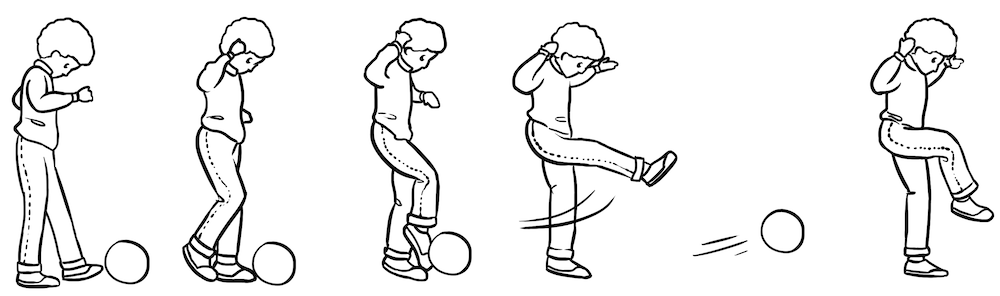
\includegraphics[keepaspectratio]{static/images/man-kick/ki1.png}}
& \textbf{Level 1}The child stands behind the ball and kicks it without
stepping forward. \\
\pandocbounded{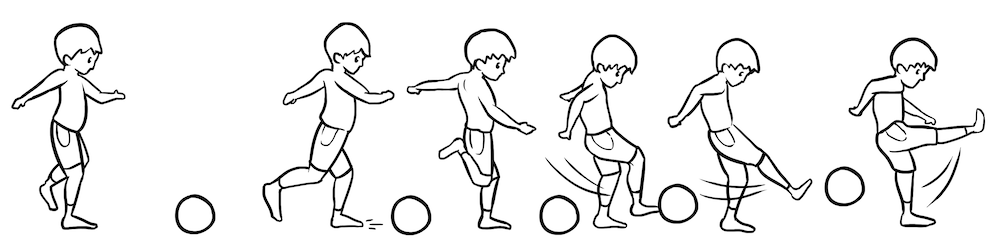
\includegraphics[keepaspectratio]{static/images/man-kick/ki2.png}}
& \textbf{Level 2}At least one step is taken before kicking the ball
without a long stride or leap. It often appears as though the child runs
directly through the ball. \\
\pandocbounded{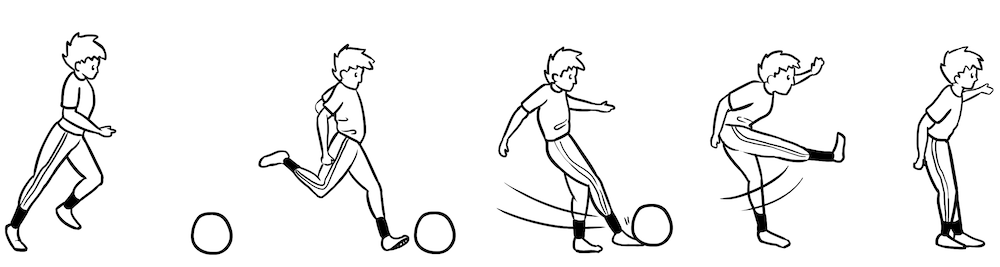
\includegraphics[keepaspectratio]{static/images/man-kick/ki3.png}}
& \textbf{Level 3}Before kicking, there are a few steps toward the ball
with a lengthened stride or jump. However, there is no follow-through
after the kick. \\
\pandocbounded{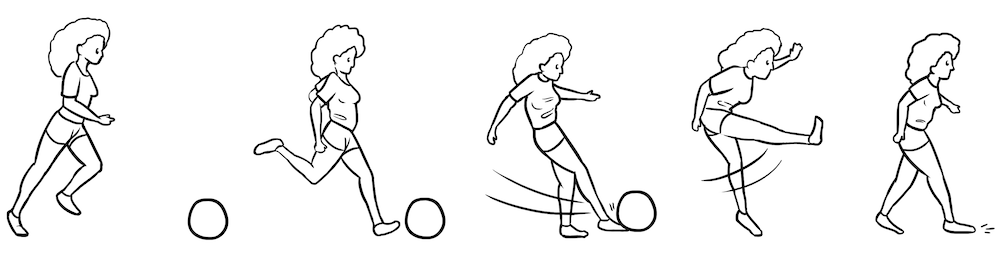
\includegraphics[keepaspectratio]{static/images/man-kick/ki4.png}}
& \textbf{Level 4}There is a long stride or leap before contacting the
ball. After contact, the placement foot continues moving forward. \\
\end{longtable}

\section{Dribble}\label{dribble}

\subsection{Equipment}\label{equipment-3}

\begin{itemize}
\tightlist
\item
  Small and medium-sized basketballs
\item
  Basket
\item
  Floor tape
\item
  stopwatch
\end{itemize}

\subsection{Setup}\label{setup-2}

\begin{itemize}
\tightlist
\item
  Tape a 4' x 4' square on the floor to designate personal space.
\item
  Stand about 6 feet from the examinee.
\item
  Have a bucket with several soccer balls inside, placed 3 feet before
  the kicking line.
\end{itemize}

\subsection{Directions for
performers}\label{directions-for-performers-2}

\begin{itemize}
\tightlist
\item
  I want to see you dribbling a basketball with one hand.
\item
  Try to stay inside the square while dribbling the ball.
\item
  If the ball goes out of bounds, pick it up, return inside the square,
  and re-start.
\item
  I will tell you when to stop.
\item
  Watch as I demonstrate.
\end{itemize}

\subsection{Notes for examiners}\label{notes-for-examiners-2}

\begin{itemize}
\tightlist
\item
  Inquire about the child's preferred foot
\item
  Give the performer a practice trial (about 5 seconds).
\item
  Use a stopwatch to time the child's dribbling for 15 seconds. Stop
  time if the ball goes out of bounce. Resume timing when the child
  restarts dribbling.
\item
  Children who can control the ball without looking demonstrate
  vision-independent control. Otherwise, they are at Level 3
\end{itemize}

\subsection{Scale}\label{scale-2}

\begin{figure}

\centering{

\pandocbounded{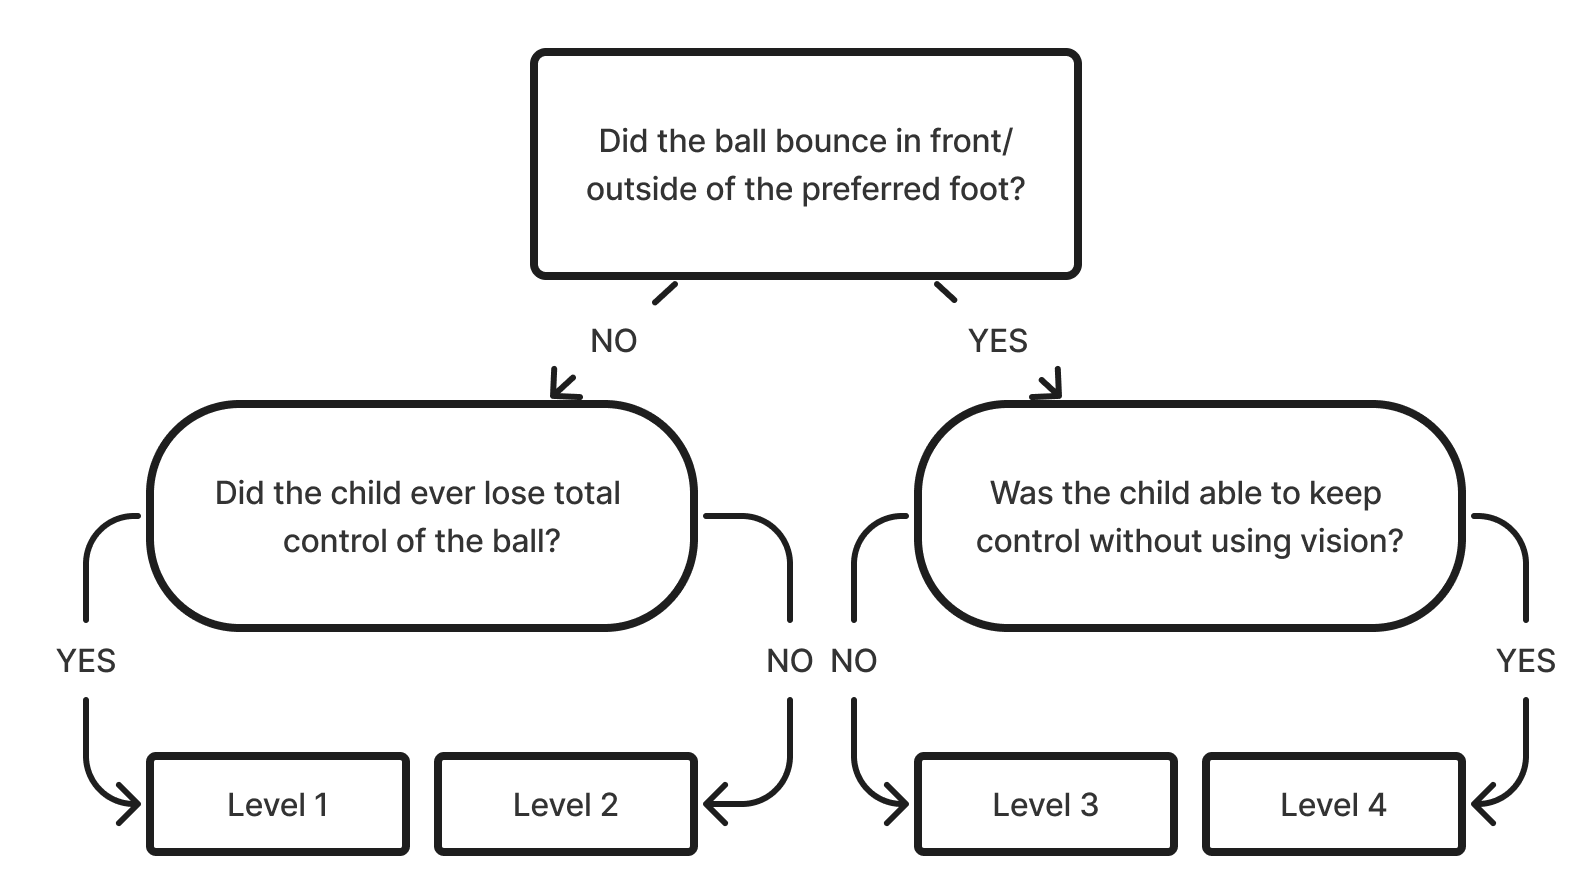
\includegraphics[keepaspectratio]{static/images/man-dribble/scale-man-dribble.png}}

}

\caption{\label{fig-scale-dribble}Scale for Dribble}

\end{figure}%

\subsection{Developmental Sequences}\label{developmental-sequences-2}

\begin{longtable}[]{@{}
  >{\centering\arraybackslash}p{(\linewidth - 2\tabcolsep) * \real{0.3500}}
  >{\raggedright\arraybackslash}p{(\linewidth - 2\tabcolsep) * \real{0.6500}}@{}}
\toprule\noalign{}
\begin{minipage}[b]{\linewidth}\centering
Image
\end{minipage} & \begin{minipage}[b]{\linewidth}\raggedright
Description
\end{minipage} \\
\midrule\noalign{}
\endhead
\bottomrule\noalign{}
\endlastfoot
\pandocbounded{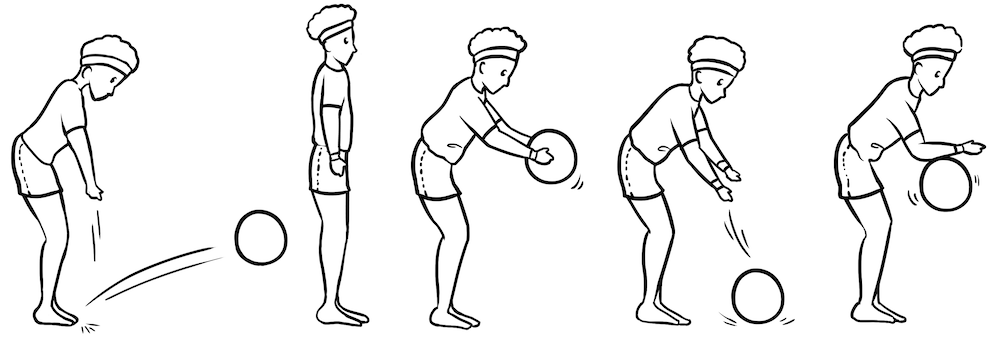
\includegraphics[keepaspectratio]{static/images/man-dribble/dr1.png}}
& \textbf{Level 1}The child struggles to control the ball as it bounces
erratically and loses control at least once. \\
\pandocbounded{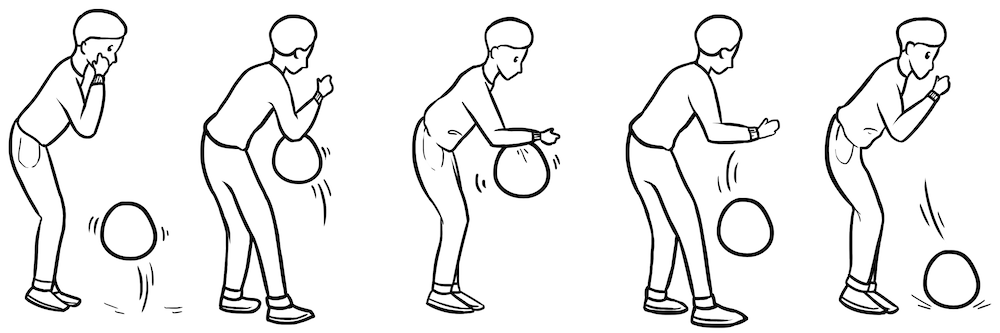
\includegraphics[keepaspectratio]{static/images/man-dribble/dr2.png}}
& \textbf{Level 2}Despite a lack of control, the child bounces the ball
continuously for 15 seconds. \\
\pandocbounded{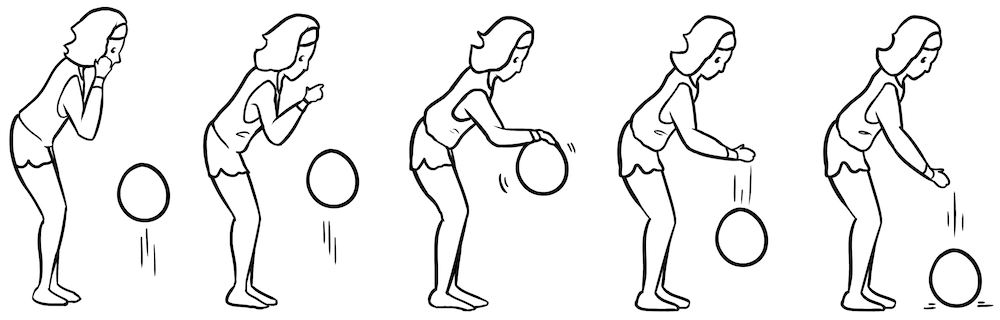
\includegraphics[keepaspectratio]{static/images/man-dribble/dr3.png}}
& \textbf{Level 3}Vision is used to maintain ball control. Bounces occur
in front of or to the outside of the child's preferred foot, and the
child has more control over the ball. \\
\pandocbounded{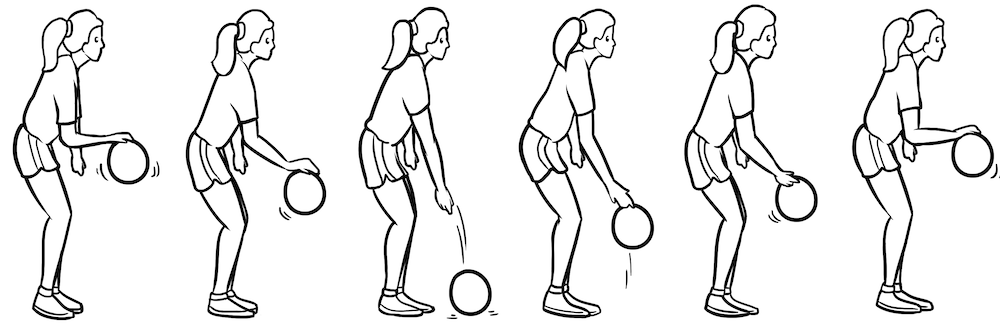
\includegraphics[keepaspectratio]{static/images/man-dribble/dr4.png}}
& \textbf{Level 4}Control is clear, and the child does not rely on
vision to maintain ball control. \\
\end{longtable}

\section{Catch}\label{catch}

\subsection{Equipment}\label{equipment-4}

\begin{itemize}
\tightlist
\item
  4- and 8-inch balls
\item
  Floor tape
\end{itemize}

\subsection{Setup}\label{setup-3}

\begin{itemize}
\tightlist
\item
  Tape a 4'x4' on the floor to designate personal space.
\item
  Stand about 6 feet from the child.
\end{itemize}

\subsection{Directions for
performers}\label{directions-for-performers-3}

\begin{itemize}
\tightlist
\item
  I want to see you catch a ball with two hands.
\item
  Stand anywhere inside the square.
\item
  Watch as I demonstrate.
\end{itemize}

\subsection{Notes for examiners}\label{notes-for-examiners-3}

\begin{itemize}
\tightlist
\item
  Give the performer four trials (the first trial is for practice only).
\item
  Use an underhand toss and toss the ball at the child's chest level.
\item
  Repeat any attempt that results from a bad toss (too high/low or to
  the sides).
\item
  Only assess consistency on the three ``valid'' tosses.
\item
  If the ball is caught with hands and later brought against the chest,
  this indicates Level 2.
\item
  A behavior is considered present (answering YES) if observed in at
  least two trials.
\item
  Use either the 4-inch or 8-inch ball, depending on the child's size
  and strength. The 4-inch ball is recommended for smaller children.
\end{itemize}

\subsection{Scale}\label{scale-3}

\begin{figure}

\centering{

\pandocbounded{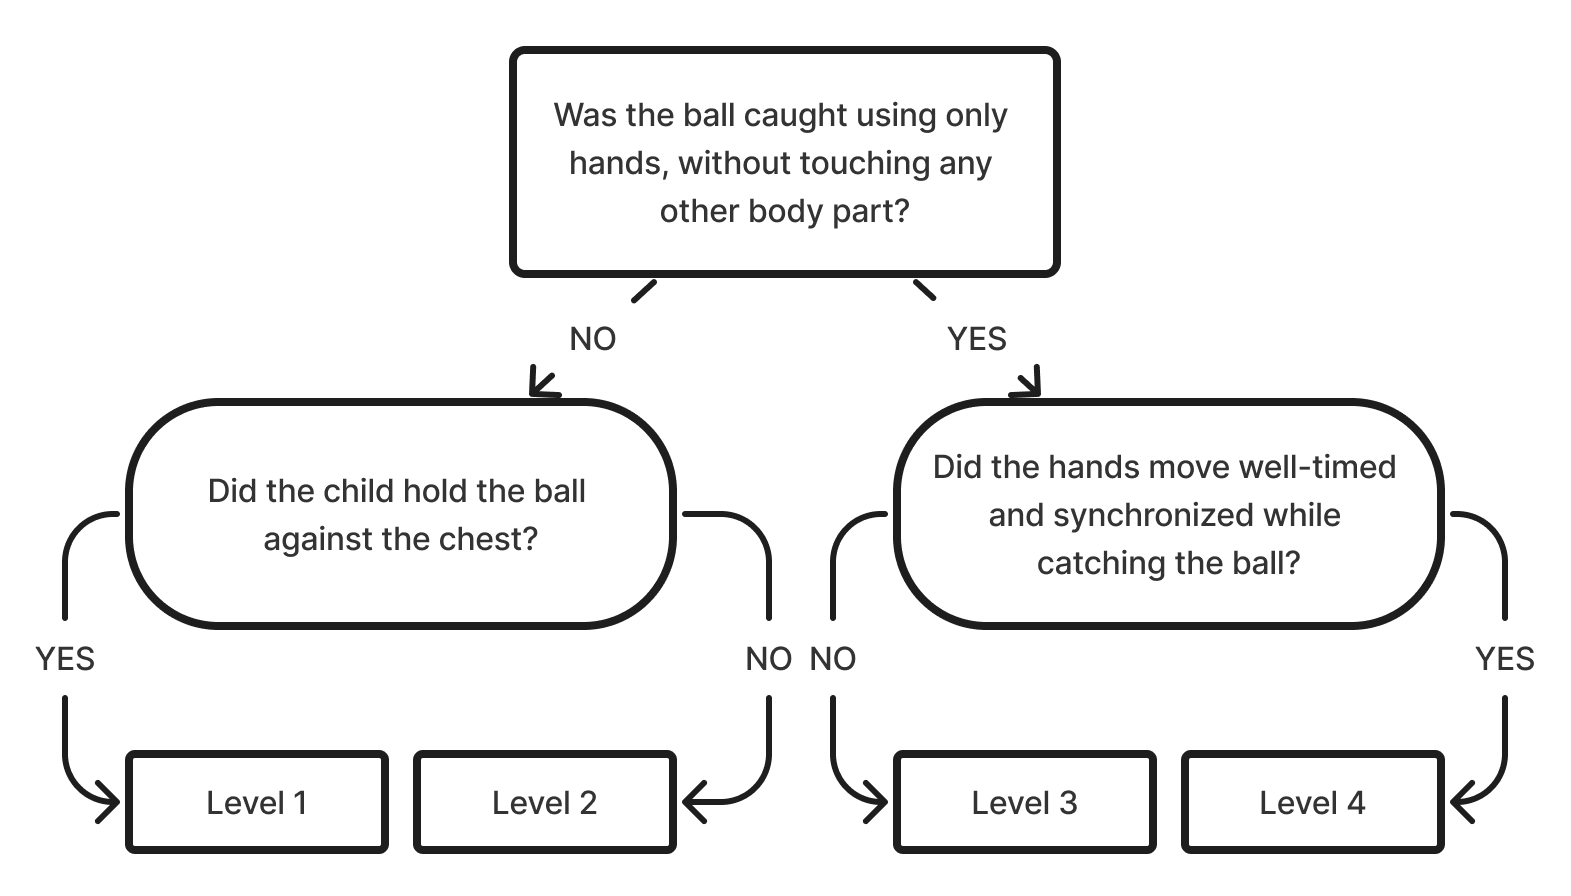
\includegraphics[keepaspectratio]{static/images/man-catch/scale-man-catch.png}}

}

\caption{\label{fig-scale-catch}Scale for Catch}

\end{figure}%

\subsection{Developmental Sequences}\label{developmental-sequences-3}

\begin{longtable}[]{@{}
  >{\raggedright\arraybackslash}p{(\linewidth - 2\tabcolsep) * \real{0.3500}}
  >{\raggedright\arraybackslash}p{(\linewidth - 2\tabcolsep) * \real{0.6500}}@{}}
\toprule\noalign{}
\begin{minipage}[b]{\linewidth}\raggedright
Image
\end{minipage} & \begin{minipage}[b]{\linewidth}\raggedright
Description
\end{minipage} \\
\midrule\noalign{}
\endhead
\bottomrule\noalign{}
\endlastfoot
\pandocbounded{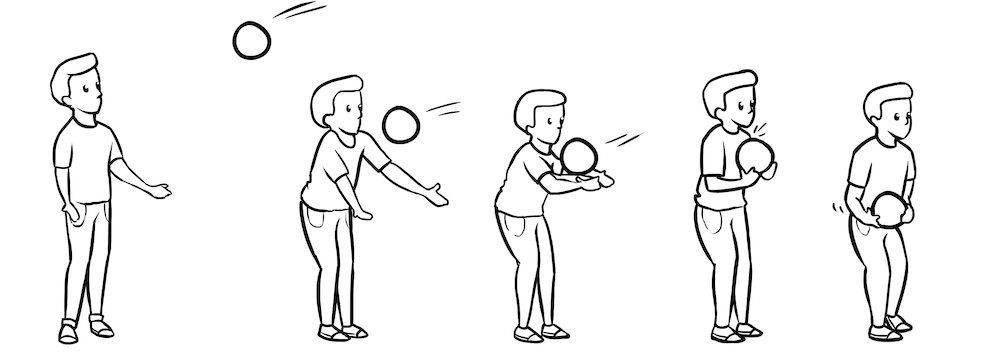
\includegraphics[keepaspectratio]{static/images/man-catch/ca1.png}}
& \textbf{Level 1}The child uses a scooping action to secure the ball
against the chest. \\
\pandocbounded{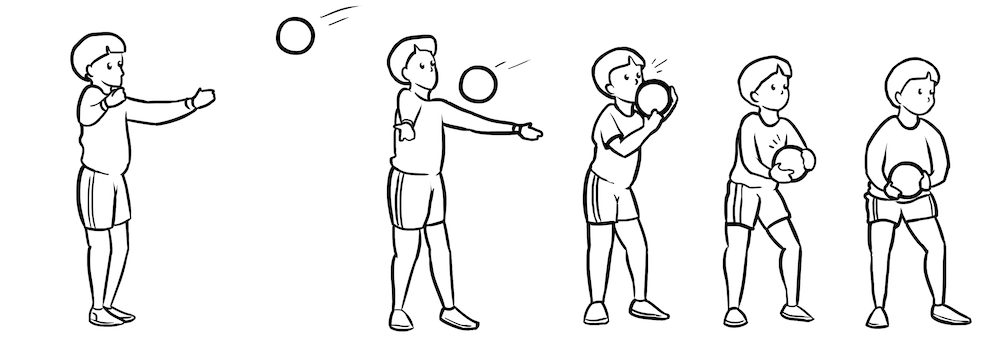
\includegraphics[keepaspectratio]{static/images/man-catch/ca2.png}}
& \textbf{Level 2}Following a successful catch, the ball is not secured
against the chest but touches a body part other than the hands. \\
\pandocbounded{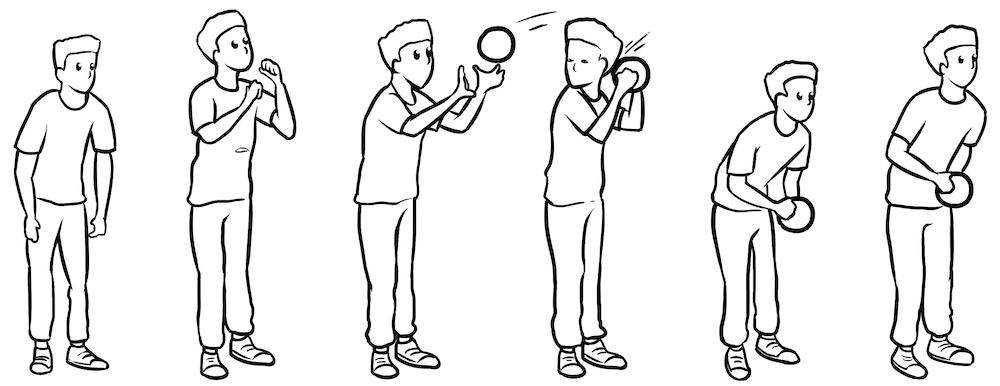
\includegraphics[keepaspectratio]{static/images/man-catch/ca3.png}}
& \textbf{Level 3}The action lacks coordination, with the ball making
contact only with the hands. Players often extend their arms and/or turn
their faces to the side. \\
\pandocbounded{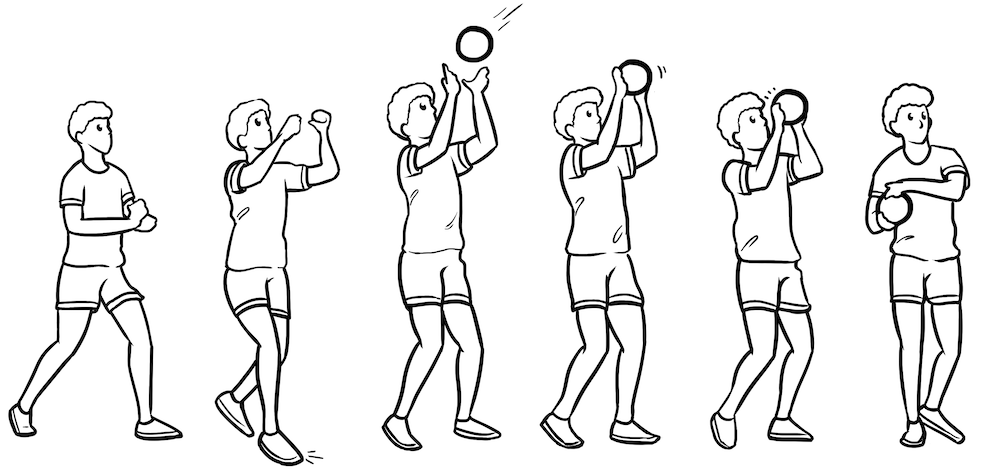
\includegraphics[keepaspectratio]{static/images/man-catch/ca4.png}}
& \textbf{Level 4}Action is well-timed with the simultaneous motion of
hands. \\
\end{longtable}

\section{Striking}\label{striking}

\subsection{Equipment}\label{equipment-5}

\begin{itemize}
\tightlist
\item
  Lightweight plastic bat
\item
  4-inch balls
\item
  Floor tape
\end{itemize}

\subsection{Setup}\label{setup-4}

\begin{itemize}
\tightlist
\item
  Tape a 4'x4' square on the floor 20 feet from the wall.
\item
  Stand slightly to the side (about 12 feet), facing the child.
\item
  Invert the position (the child faces the opposite wall/open space) if
  left-handed.
\end{itemize}

\subsection{Directions for
performers}\label{directions-for-performers-4}

\begin{itemize}
\tightlist
\item
  I want to see you strike a ball tossed in your direction.
\item
  Try to stay inside the square, but you are free to move as the ball
  approaches.
\item
  Strike the ball against the wall/open space.
\item
  Watch as I demonstrate.
\end{itemize}

\subsection{Notes for examiners}\label{notes-for-examiners-4}

\begin{itemize}
\tightlist
\item
  Give the performer 4 trials (1st trial is for practice only).
\item
  Use an underhand toss.
\item
  Toss the ball just above the child's hip level.
\item
  Repeat any attempt that results from a bad toss (too high/low or to
  the sides).
\item
  Only assess consistency on the three ``valid'' tosses.
\item
  A behavior is considered present (answering YES) if observed in at
  least two trials.
\end{itemize}

\subsection{Scale}\label{scale-4}

\begin{figure}

\centering{

\pandocbounded{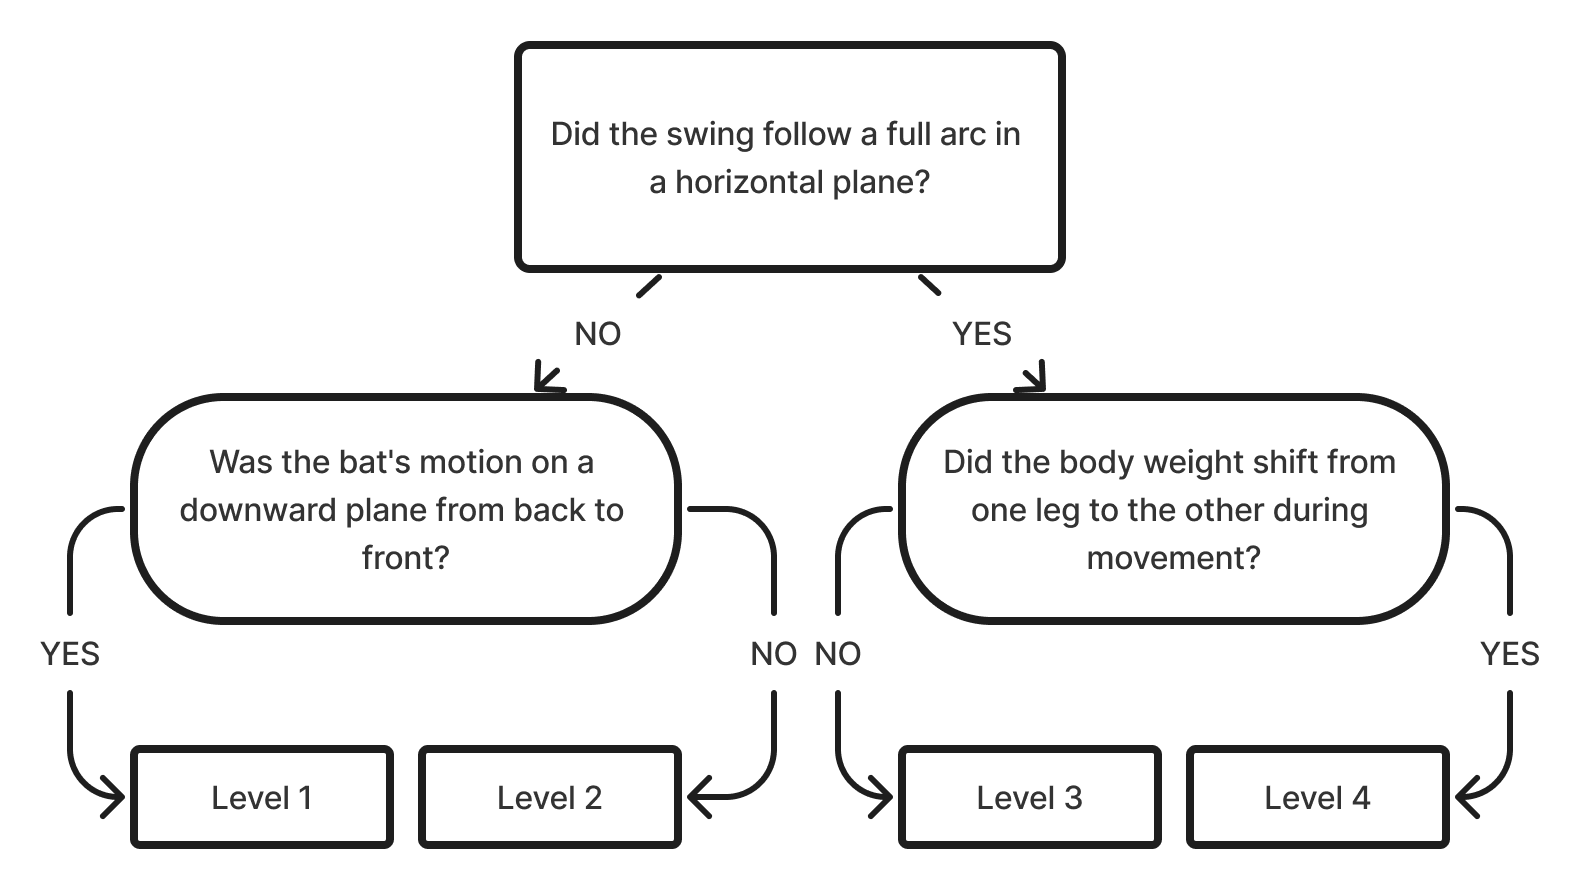
\includegraphics[keepaspectratio]{static/images/man-strike/scale-man-strike.png}}

}

\caption{\label{fig-scale-strike}Scale for Striking}

\end{figure}%

\subsection{Developmental Sequences}\label{developmental-sequences-4}

\begin{longtable}[]{@{}
  >{\raggedright\arraybackslash}p{(\linewidth - 2\tabcolsep) * \real{0.3500}}
  >{\raggedright\arraybackslash}p{(\linewidth - 2\tabcolsep) * \real{0.6500}}@{}}
\toprule\noalign{}
\begin{minipage}[b]{\linewidth}\raggedright
Image
\end{minipage} & \begin{minipage}[b]{\linewidth}\raggedright
Description
\end{minipage} \\
\midrule\noalign{}
\endhead
\bottomrule\noalign{}
\endlastfoot
\pandocbounded{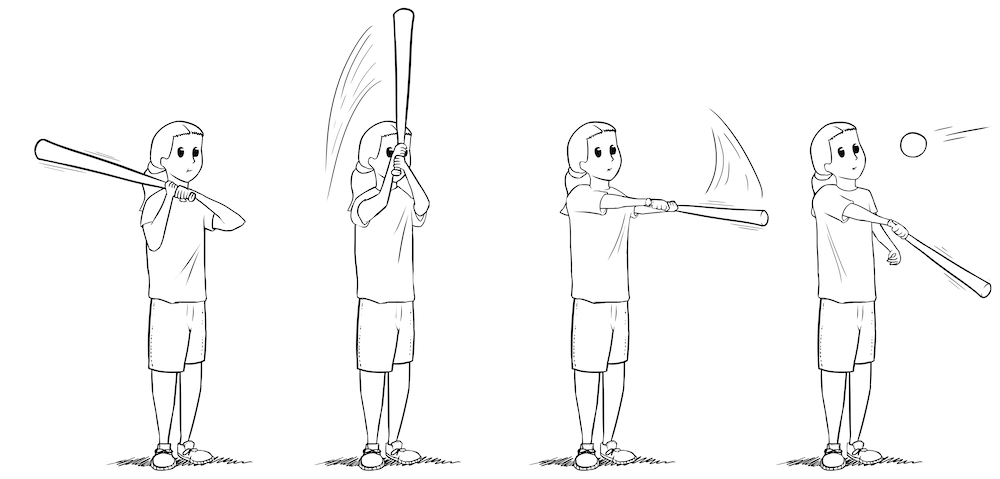
\includegraphics[keepaspectratio]{static/images/man-strike/st1.png}}
& \textbf{Level 1}The arm action is from back to front and resembles a
vertical chopping motion. \\
\pandocbounded{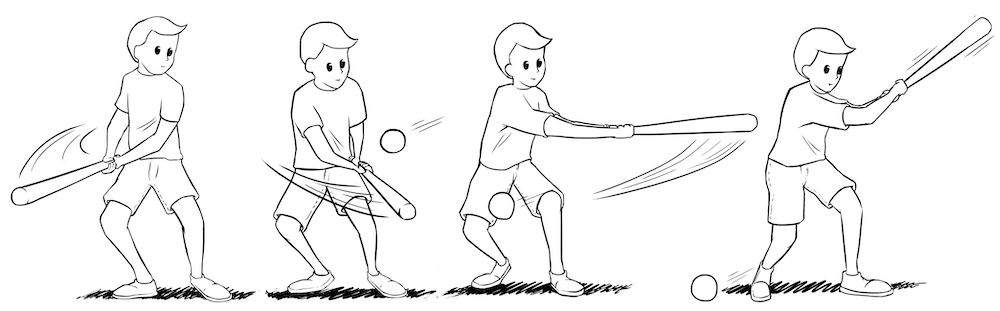
\includegraphics[keepaspectratio]{static/images/man-strike/st2.png}}
& \textbf{Level 2}The motion occurs on the horizontal plane, but the
action is limited in its amplitude. Often, the bat is held in front of
the body. \\
\pandocbounded{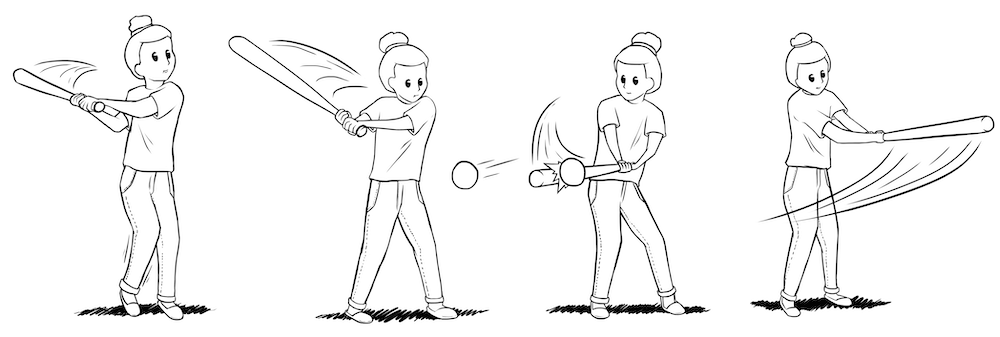
\includegraphics[keepaspectratio]{static/images/man-strike/st3.png}}
& \textbf{Level 3}The strike does occur in a long (full arc) horizontal
plan, but there is no body weight transfer. \\
\pandocbounded{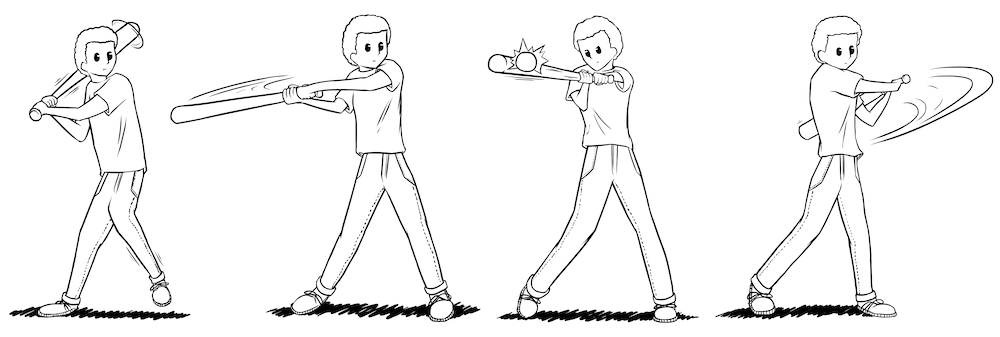
\includegraphics[keepaspectratio]{static/images/man-strike/st4.png}}
& \textbf{Level 4}Same as Level 3, but now there is a transfer of body
weight in the direction of the strike, which occurs from one to the
other leg. \\
\end{longtable}

\bookmarksetup{startatroot}

\chapter{Locomotor Subscale}\label{locomotor-subscale}

\section{Hop}\label{hop}

\subsection{Equipment}\label{equipment-6}

\begin{itemize}
\tightlist
\item
  Plastic cones
\item
  Floor tape
\end{itemize}

\subsection{Setup}\label{setup-5}

\begin{itemize}
\tightlist
\item
  Create a 15-long traveling lane using cones.
\item
  Tape starting and ending lines on the floor.
\item
  Stand perpendicular to the traveling lane to see the starting and
  ending points.
\item
  Place two cones (each end) 1 foot before the starting and ending
  lines.
\end{itemize}

\subsection{Directions for
performers}\label{directions-for-performers-5}

\begin{itemize}
\tightlist
\item
  I want to see you hopping on one leg.
\item
  Choose your preferred leg to hop.
\item
  Start from that starting line and do not stop until you pass the
  ending line; then come back using the same leg.
\item
  This is not a race; show your best form.
\item
  Watch as I demonstrate.
\end{itemize}

\subsection{Notes for examiners}\label{notes-for-examiners-5}

\begin{itemize}
\tightlist
\item
  Give the performer 4 trials (1st trial is for practice only).
\item
  A behavior is considered present (answering YES) if observed in at
  least two trials.
\end{itemize}

\subsection{Scale}\label{scale-5}

\begin{figure}

\centering{

\pandocbounded{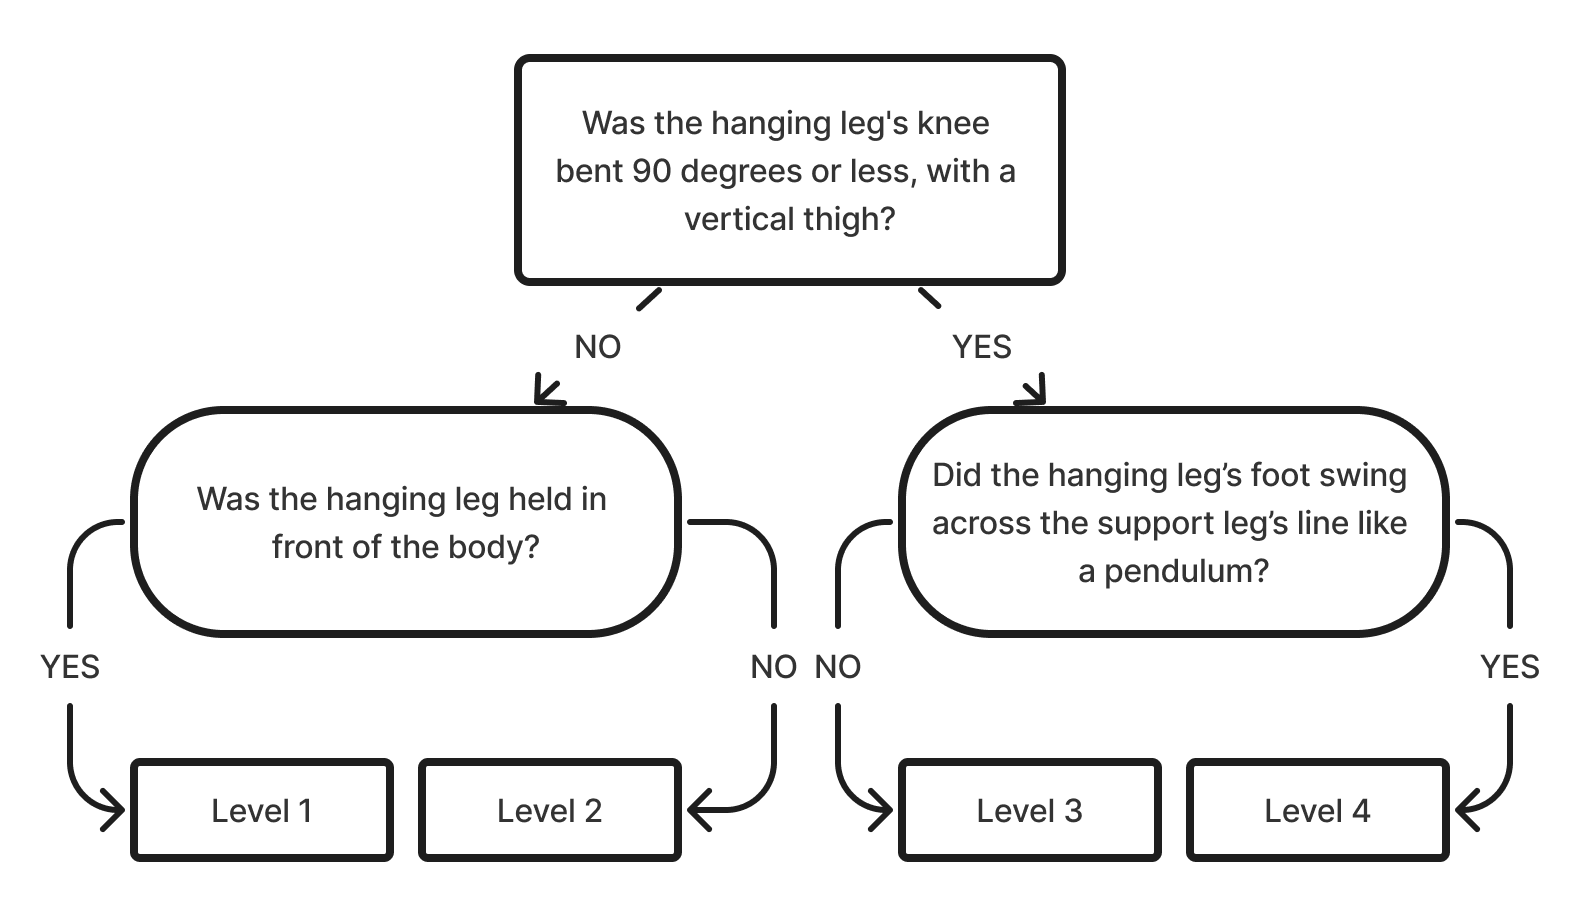
\includegraphics[keepaspectratio]{static/images/loc-hop/scale-loc-hop.png}}

}

\caption{\label{fig-scale-hop}Scale for Hop}

\end{figure}%

\subsection{Developmental Sequences}\label{developmental-sequences-5}

\begin{longtable}[]{@{}
  >{\raggedright\arraybackslash}p{(\linewidth - 2\tabcolsep) * \real{0.3500}}
  >{\raggedright\arraybackslash}p{(\linewidth - 2\tabcolsep) * \real{0.6500}}@{}}
\toprule\noalign{}
\begin{minipage}[b]{\linewidth}\raggedright
Image
\end{minipage} & \begin{minipage}[b]{\linewidth}\raggedright
Description
\end{minipage} \\
\midrule\noalign{}
\endhead
\bottomrule\noalign{}
\endlastfoot
\pandocbounded{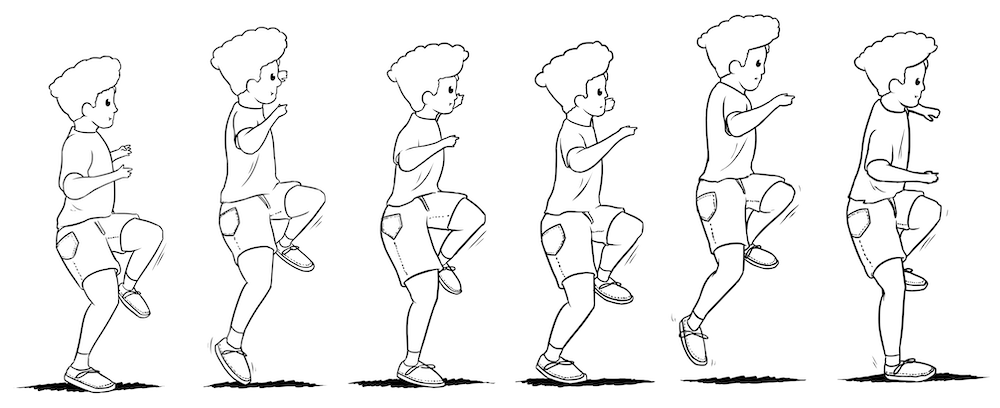
\includegraphics[keepaspectratio]{static/images/loc-hop/ho1.png}}
& \textbf{Level 1}The suspended leg is held in front of the body. \\
\pandocbounded{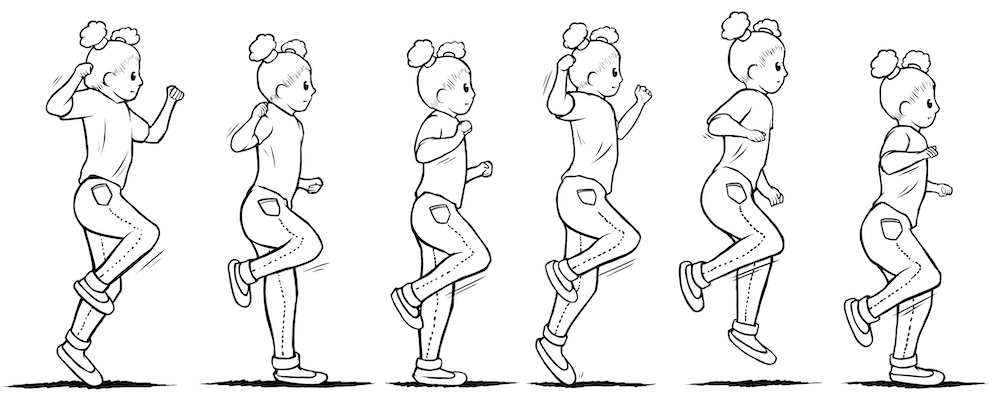
\includegraphics[keepaspectratio]{static/images/loc-hop/ho2.png}}
& \textbf{Level 2}The knee is flexed with the foot of the hanging leg
held near the buttocks. \\
\pandocbounded{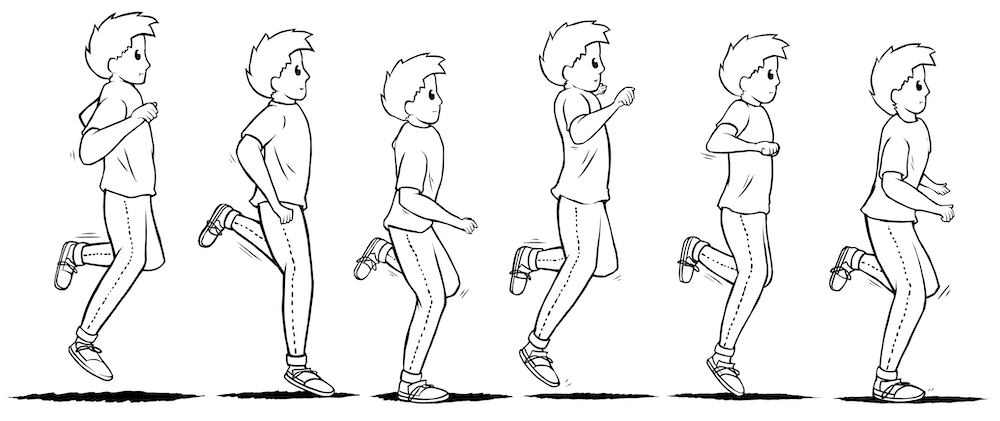
\includegraphics[keepaspectratio]{static/images/loc-hop/ho3.png}}
& \textbf{Level 3}The hanging leg is held back with the thigh
vertically. \\
\pandocbounded{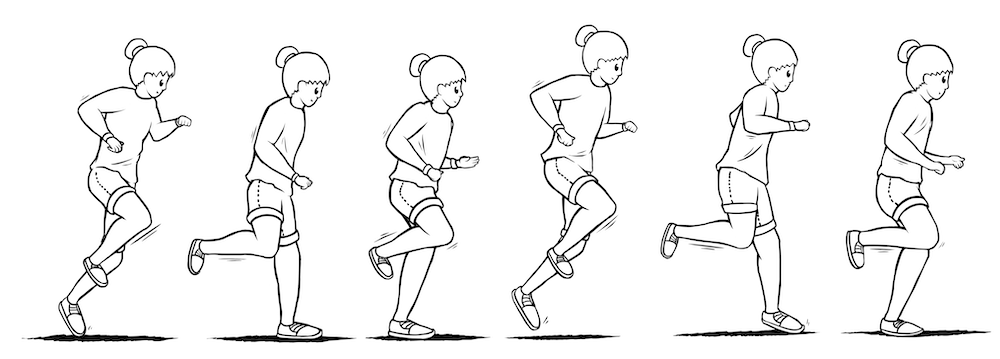
\includegraphics[keepaspectratio]{static/images/loc-hop/ho4.png}}
& \textbf{Level 4}Similar to Level 3, the foot of the hanging leg
crosses the line of the support leg like a pendulum. \\
\end{longtable}

\section{Horizontal Jump}\label{horizontal-jump}

\subsection{Equipment}\label{equipment-7}

\begin{itemize}
\tightlist
\item
  Floor tape
\item
  Plastic cones
\end{itemize}

\subsection{Setup}\label{setup-6}

\begin{itemize}
\tightlist
\item
  Tape two parallel lines on the floor two feet apart.
\item
  Stand perpendicular to the jumping action facing the side of the
  child.
\end{itemize}

\subsection{Directions for
performers}\label{directions-for-performers-6}

\begin{itemize}
\tightlist
\item
  I want to see you jumping forward over the second line and using both
  feet.
\item
  Walk up to the first line and stop completely.
\item
  Then, jump as far as you can over the second line.
\item
  Use both feet when taking off and landing.
\item
  Then, walk back to the starting point and do it again.
\item
  There is no rush; show your best jump.
\item
  Watch as I demonstrate.
\end{itemize}

\subsection{Notes for examiners}\label{notes-for-examiners-6}

\begin{itemize}
\tightlist
\item
  Give the performer 4 trials (1st trial is for practice only).
\item
  The child must stop completely behind the line before jumping.
\end{itemize}

\subsection{Scale}\label{scale-6}

\begin{figure}

\centering{

\pandocbounded{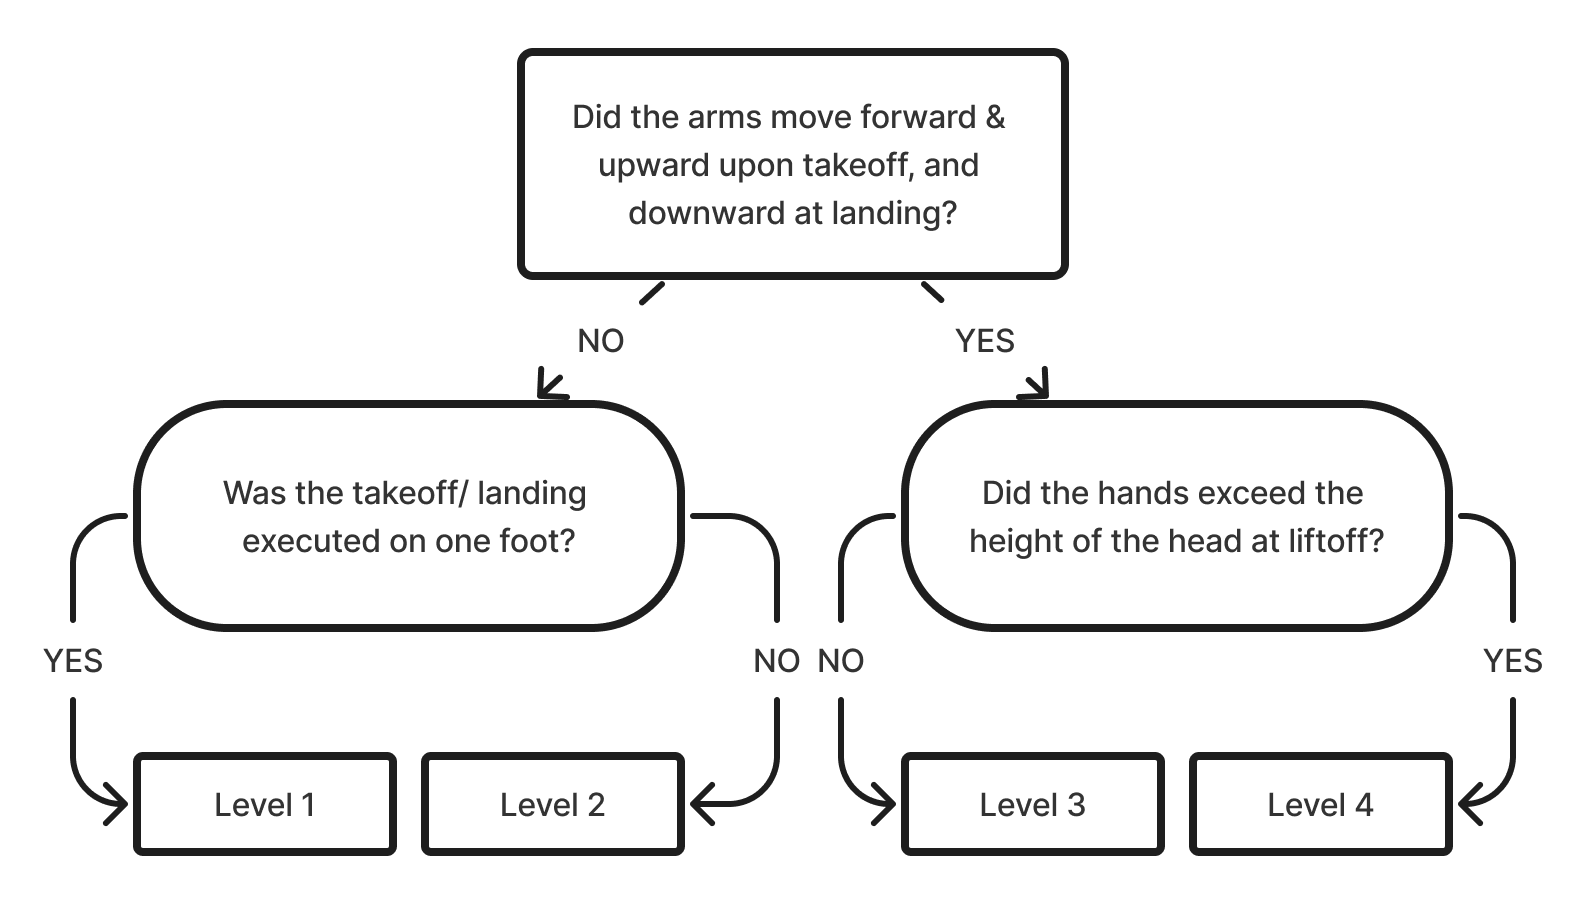
\includegraphics[keepaspectratio]{static/images/loc-hj/scale-loc-hj.png}}

}

\caption{\label{fig-scale-hj}Scale for Horizontal Jump}

\end{figure}%

\subsection{Developmental Sequences}\label{developmental-sequences-6}

\begin{longtable}[]{@{}
  >{\raggedright\arraybackslash}p{(\linewidth - 2\tabcolsep) * \real{0.3500}}
  >{\raggedright\arraybackslash}p{(\linewidth - 2\tabcolsep) * \real{0.6500}}@{}}
\toprule\noalign{}
\begin{minipage}[b]{\linewidth}\raggedright
Image
\end{minipage} & \begin{minipage}[b]{\linewidth}\raggedright
Description
\end{minipage} \\
\midrule\noalign{}
\endhead
\bottomrule\noalign{}
\endlastfoot
\pandocbounded{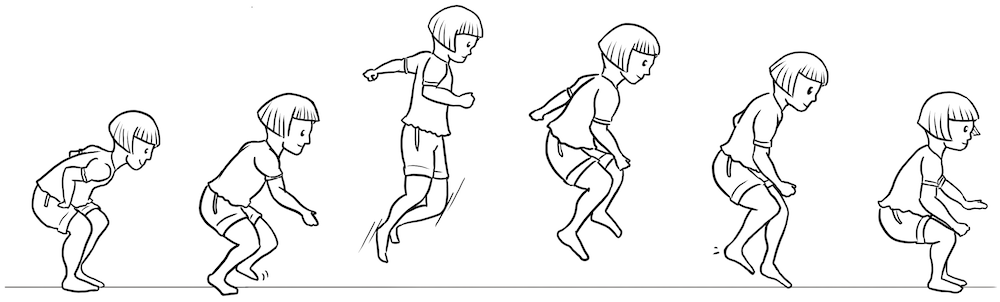
\includegraphics[keepaspectratio]{static/images/loc-hj/hj1.png}}
& \textbf{Level 1}The arm action is inconsistent with no defined
pattern, sometimes even motionless. The takeoff and/or landing is
executed on one foot. \\
\pandocbounded{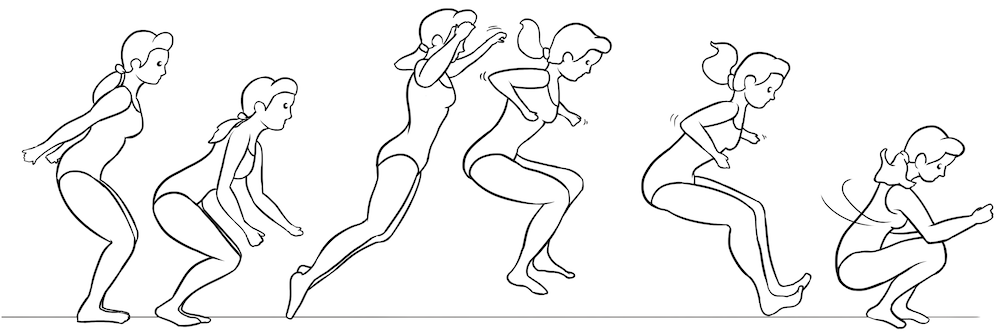
\includegraphics[keepaspectratio]{static/images/loc-hj/hj2.png}}
& \textbf{Level 2}The arm action may still be inconsistent, but the
takeoff/landing is executed on both feet. \\
\pandocbounded{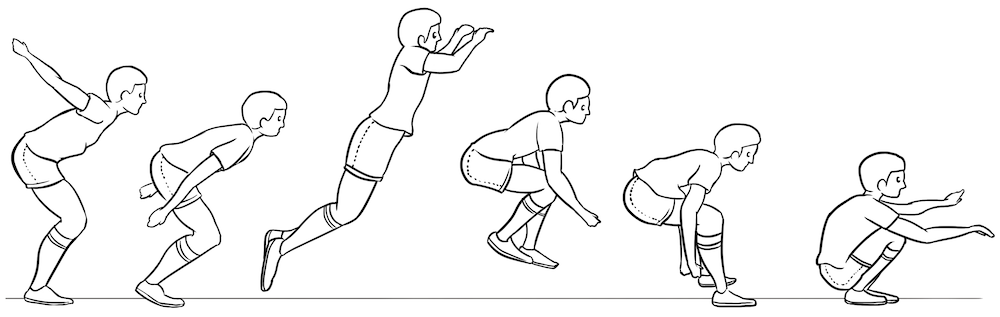
\includegraphics[keepaspectratio]{static/images/loc-hj/hj3.png}}
& \textbf{Level 3}The arms move forward and upward during takeoff and
then downward at landing. But the hands do not exceed the height of the
head at liftoff. \\
\pandocbounded{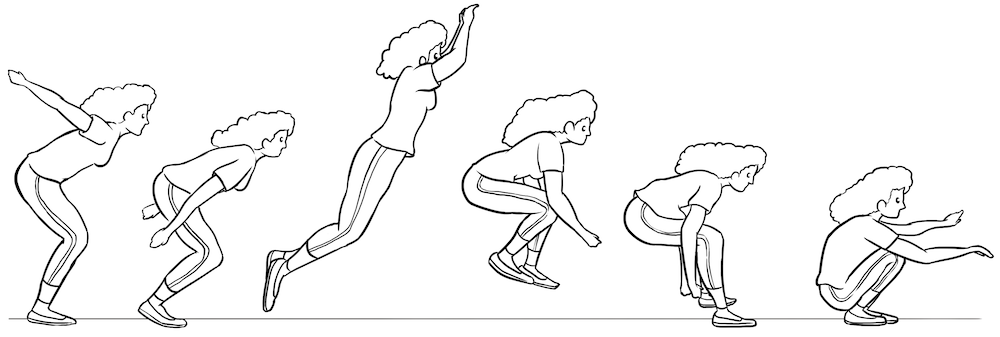
\includegraphics[keepaspectratio]{static/images/loc-hj/hj4.png}}
& \textbf{Level 4}A pattern similar to Level 3, but the hands are high
above the head during the liftoff. \\
\end{longtable}

\section{Skip}\label{skip}

\subsection{Equipment}\label{equipment-8}

\begin{itemize}
\tightlist
\item
  Plastic cones
\item
  Floor tape
\end{itemize}

\subsection{Setup}\label{setup-7}

\begin{itemize}
\tightlist
\item
  Create a 15-long traveling lane using cones.
\item
  Tape starting and ending lines on the floor.
\item
  Stand perpendicular to the traveling lane so that you can see both the
  starting and ending points.
\item
  Place two cones (each end) 1 foot before the starting and ending
  lines.
\end{itemize}

\subsection{Directions for
performers}\label{directions-for-performers-7}

\begin{itemize}
\tightlist
\item
  I want to see you skipping.
\item
  Start from that starting line and do not stop until you pass the
  ending line.
\item
  This is not a race; show your best form.
\item
  Watch as I demonstrate.
\end{itemize}

\subsection{Notes for examiners}\label{notes-for-examiners-7}

\begin{itemize}
\tightlist
\item
  Give the performer 4 trials (1st trial is for practice only).
\item
  A behavior is considered present (answering YES) if observed in at
  least two trials.
\end{itemize}

\subsection{Scale}\label{scale-7}

\begin{figure}

\centering{

\pandocbounded{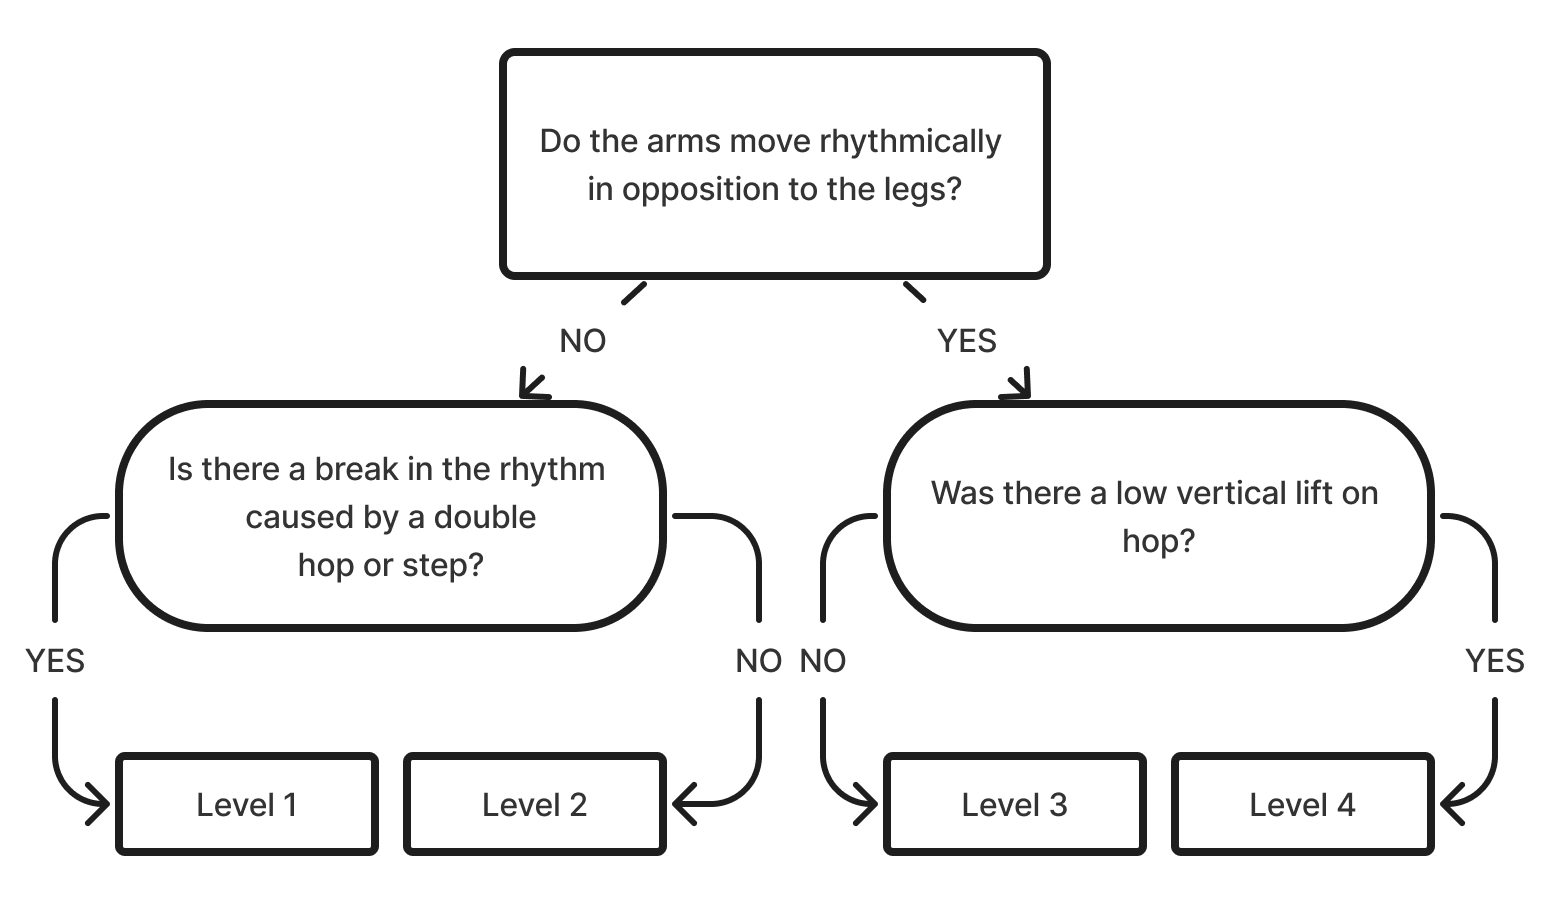
\includegraphics[keepaspectratio]{static/images/loc-skip/scale-loc-skip.png}}

}

\caption{\label{fig-scale-skip}Scale for Skip}

\end{figure}%

\subsection{Developmental Sequences}\label{developmental-sequences-7}

\begin{longtable}[]{@{}
  >{\raggedright\arraybackslash}p{(\linewidth - 2\tabcolsep) * \real{0.3500}}
  >{\raggedright\arraybackslash}p{(\linewidth - 2\tabcolsep) * \real{0.6500}}@{}}
\toprule\noalign{}
\begin{minipage}[b]{\linewidth}\raggedright
Image
\end{minipage} & \begin{minipage}[b]{\linewidth}\raggedright
Description
\end{minipage} \\
\midrule\noalign{}
\endhead
\bottomrule\noalign{}
\endlastfoot
\pandocbounded{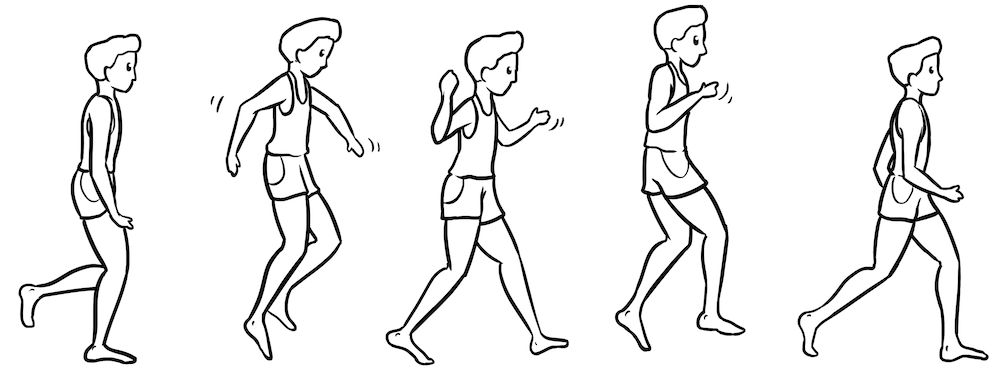
\includegraphics[keepaspectratio]{static/images/loc-skip/sk1.png}}
& \textbf{Level 1}The arm action is inconsistent, with no defined
pattern. A double hop or step affects the rhythm. \\
\pandocbounded{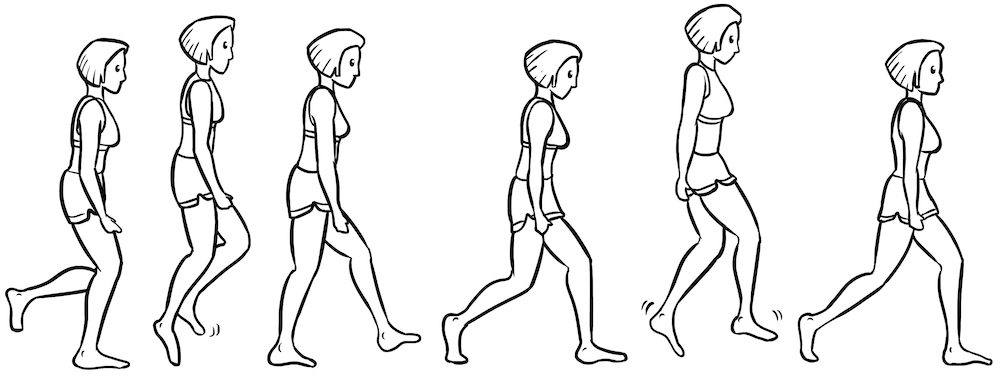
\includegraphics[keepaspectratio]{static/images/loc-skip/sk2.png}}
& \textbf{Level 2}The arm motion may improve, but it is still
inconsistent and often motionless. The action of the feet is well
coordinated and not affected by a double hop or step. \\
\pandocbounded{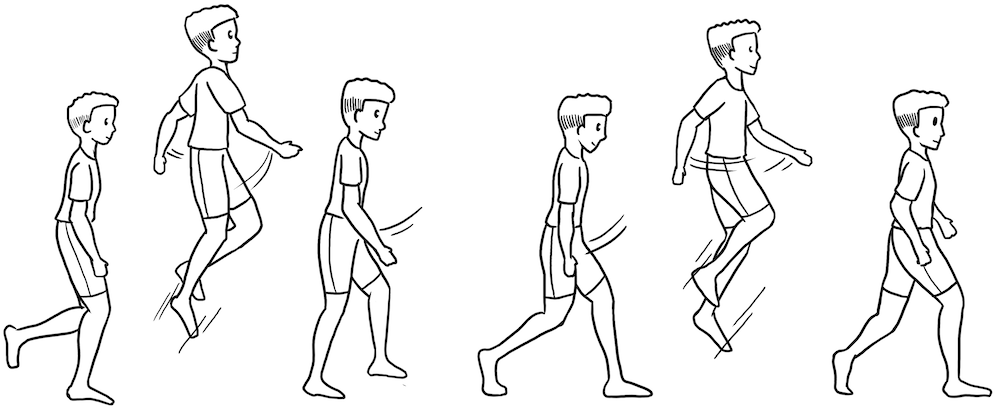
\includegraphics[keepaspectratio]{static/images/loc-skip/sk3.png}}
& \textbf{Level 3}Arms move rhythmically in opposition to the legs, but
the hop has an exaggerated vertical lift. \\
\pandocbounded{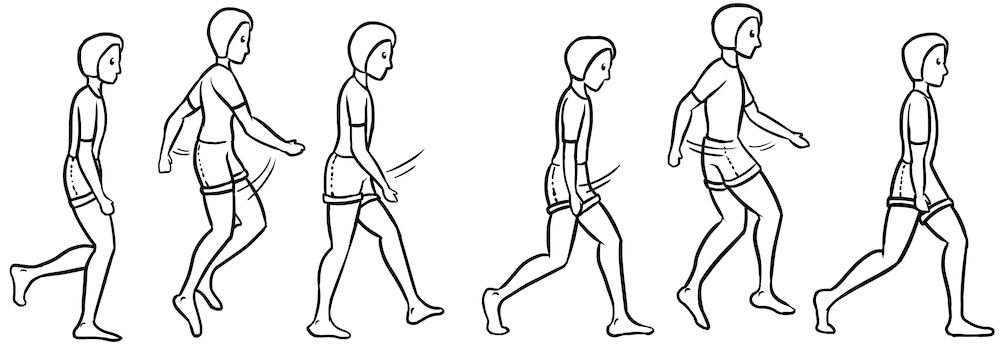
\includegraphics[keepaspectratio]{static/images/loc-skip/sk4.png}}
& \textbf{Level 4}The arms move rhythmically in opposition to the legs,
and the vertical lift on the hop is low. \\
\end{longtable}

\section{Vertical Jump}\label{vertical-jump}

\subsection{Equipment}\label{equipment-9}

\begin{itemize}
\tightlist
\item
  Floor tape
\end{itemize}

\subsection{Setup}\label{setup-8}

\begin{itemize}
\tightlist
\item
  Tape four parallel lines on the wall two feet apart.
\item
  Stand perpendicular to the jumping action, facing the side of the
  performer.
\item
  Ask the child to stand sideways with the dominant arm facing the wall.
\end{itemize}

\subsection{Directions for
performers}\label{directions-for-performers-8}

\begin{itemize}
\tightlist
\item
  I want to see you jump high.
\item
  Walk up to the wall and stand sideways.
\item
  When I say so, jump up and touch the highest point on the wall using
  your dominant hand.
\item
  Use both feet when taking off and landing.
\item
  Then, get back to the starting position.
\item
  There is no rush; show your best jump.
\item
  Watch as I demonstrate.
\end{itemize}

\subsection{Notes for examiners}\label{notes-for-examiners-8}

-Give the performer 4 trials (1st trial is for practice only). - Ask the
child to show the hand he/she writes with. That will help determine the
dominant hand.

\subsection{Scale}\label{scale-8}

\begin{figure}

\centering{

\pandocbounded{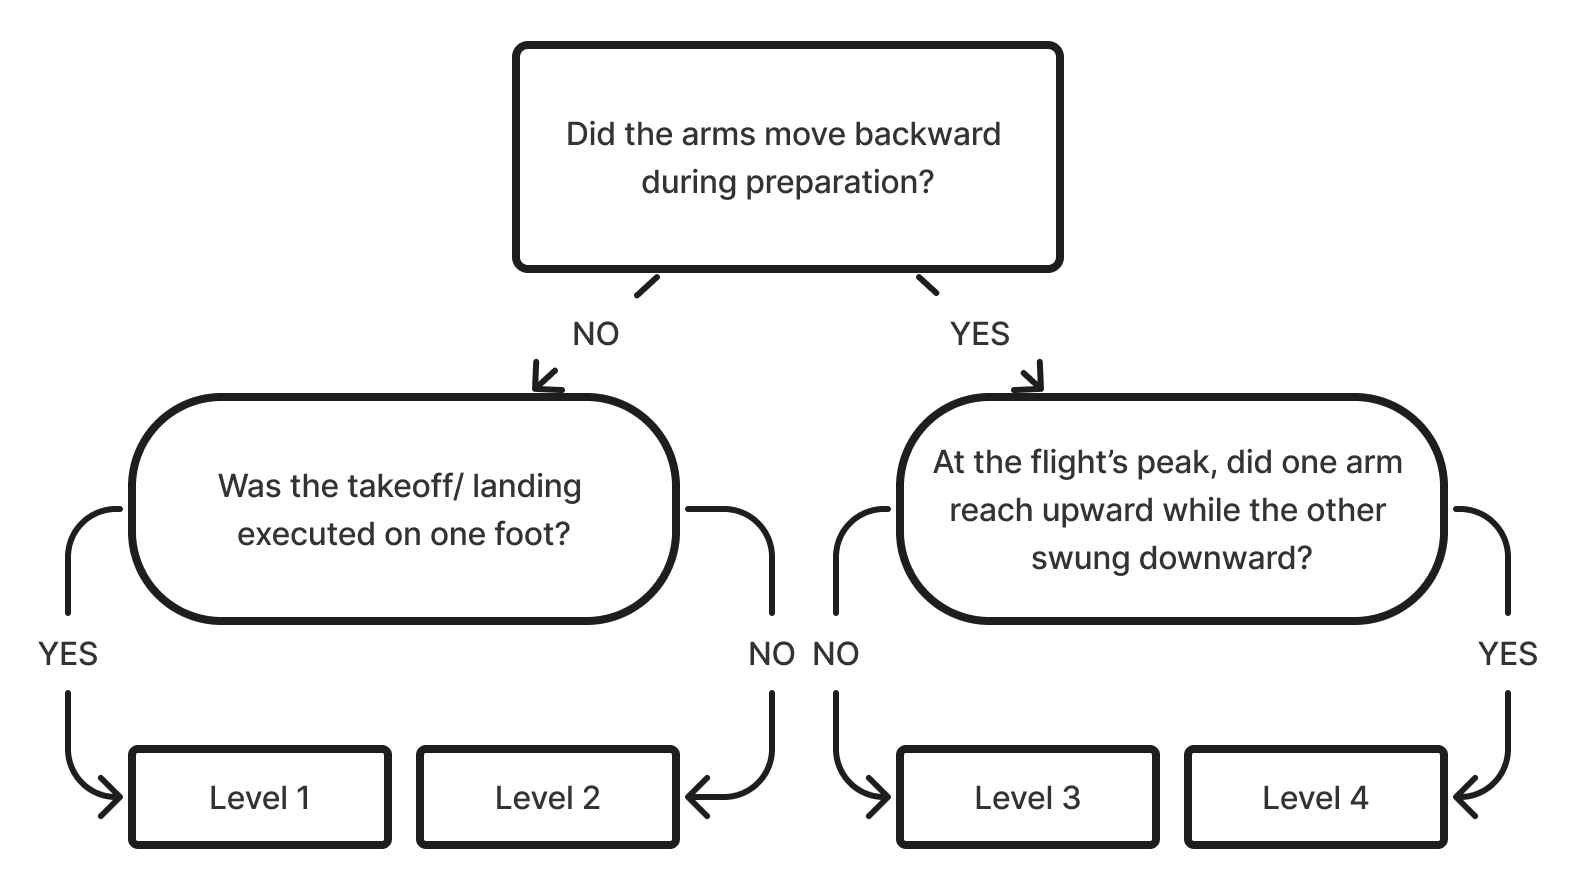
\includegraphics[keepaspectratio]{static/images/loc-vj/scale-loc-vj.png}}

}

\caption{\label{fig-scale-vj}Scale for Vertical Jump}

\end{figure}%

\subsection{Developmental Sequences}\label{developmental-sequences-8}

\begin{longtable}[]{@{}
  >{\raggedright\arraybackslash}p{(\linewidth - 2\tabcolsep) * \real{0.3500}}
  >{\raggedright\arraybackslash}p{(\linewidth - 2\tabcolsep) * \real{0.6500}}@{}}
\toprule\noalign{}
\begin{minipage}[b]{\linewidth}\raggedright
Image
\end{minipage} & \begin{minipage}[b]{\linewidth}\raggedright
Description
\end{minipage} \\
\midrule\noalign{}
\endhead
\bottomrule\noalign{}
\endlastfoot
\pandocbounded{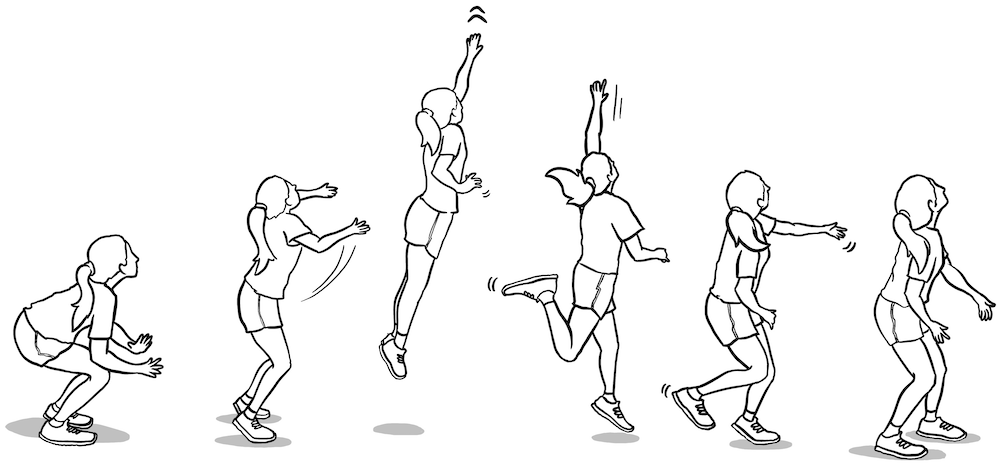
\includegraphics[keepaspectratio]{static/images/loc-vj/vj1.png}}
& \textbf{Level 1}The arms don't move to the rear before taking off; the
child takes off and/or lands with one foot. \\
\pandocbounded{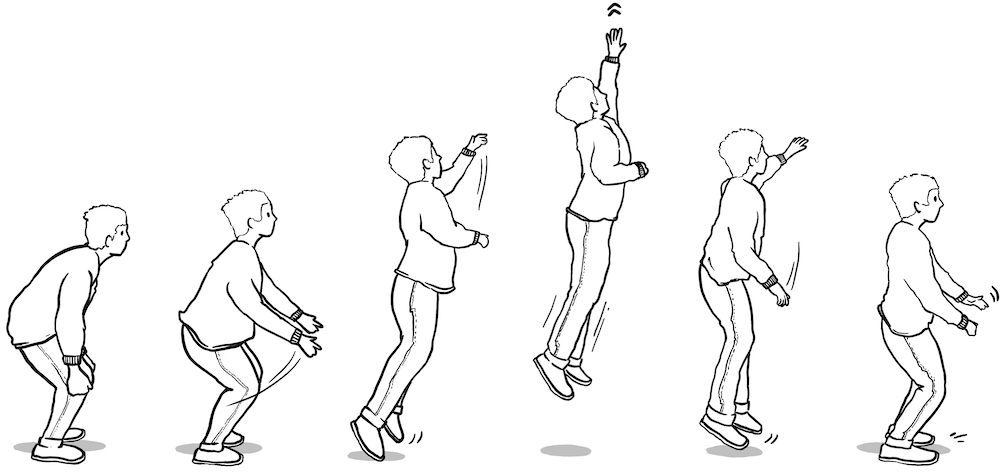
\includegraphics[keepaspectratio]{static/images/loc-vj/vj2.png}}
& \textbf{Level 2}Arms don't move to the rear before takeoff; takeoff
and landing occur with both feet. \\
\pandocbounded{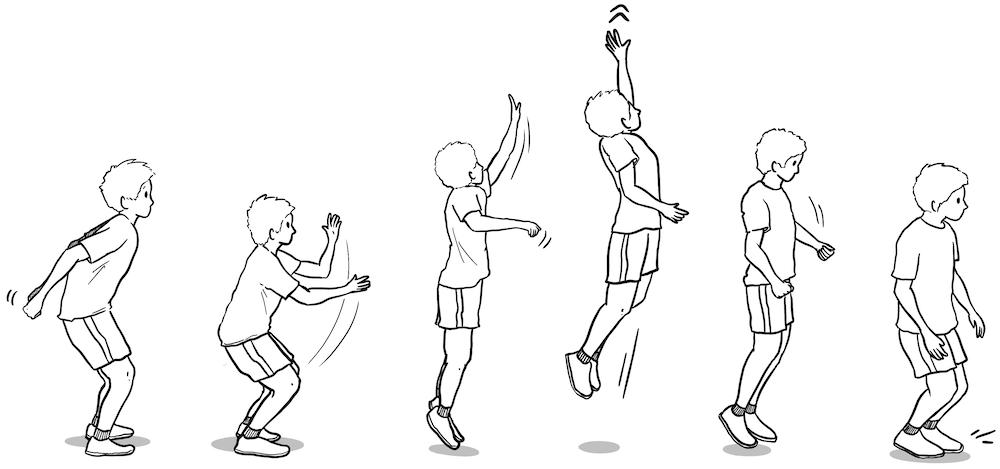
\includegraphics[keepaspectratio]{static/images/loc-vj/vj3.png}}
& \textbf{Level 3}Arms move to the rear before taking off, but only the
reaching arm reaches up. \\
\pandocbounded{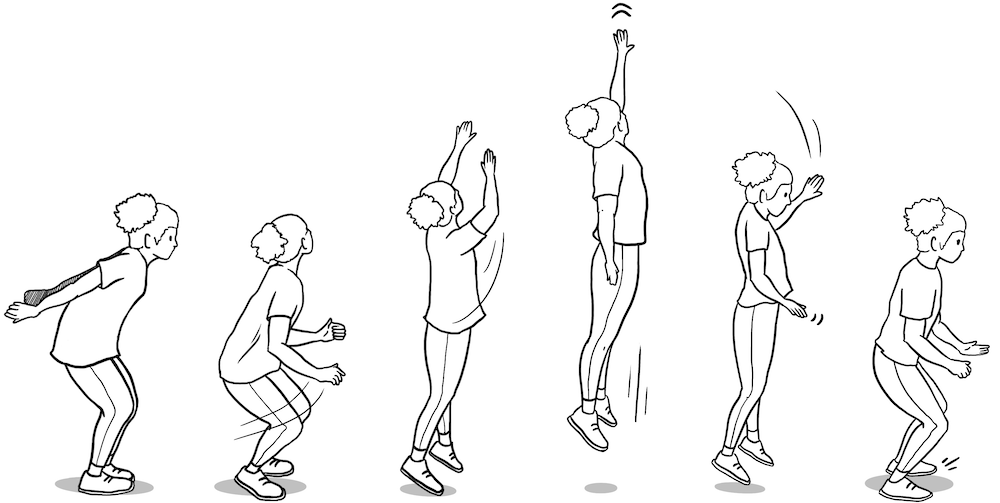
\includegraphics[keepaspectratio]{static/images/loc-vj/vj4.png}}
& \textbf{Level 4}Arms move to the rear before taking off; both arms
reach up, with the non-reaching arm moving down at the peak of the
flight. \\
\end{longtable}

\section{Gallop}\label{gallop}

\subsection{Equipment}\label{equipment-10}

\begin{itemize}
\tightlist
\item
  Floor tape
\item
  Plastic cones
\end{itemize}

\subsection{Setup}\label{setup-9}

\begin{itemize}
\tightlist
\item
  Create a 15-long traveling lane using plastic cones.
\item
  Tape starting and ending lines on the floor.
\item
  Stand perpendicular to the traveling lane so that you can see both the
  starting and ending points.
\item
  Place two cones (each end) 1 foot before the starting and ending
  lines.
\end{itemize}

\subsection{Directions for
performers}\label{directions-for-performers-9}

\begin{itemize}
\tightlist
\item
  I want to see you galloping.
\item
  Start from the starting line and do not stop until you pass the ending
  line.
\item
  This is not a race; show your best form.
\item
  Watch as I demonstrate.
\end{itemize}

\subsection{Notes for examiners}\label{notes-for-examiners-9}

Give the performer 4 trials (1st trial is for practice only).

\subsection{Scale}\label{scale-9}

\begin{figure}

\centering{

\pandocbounded{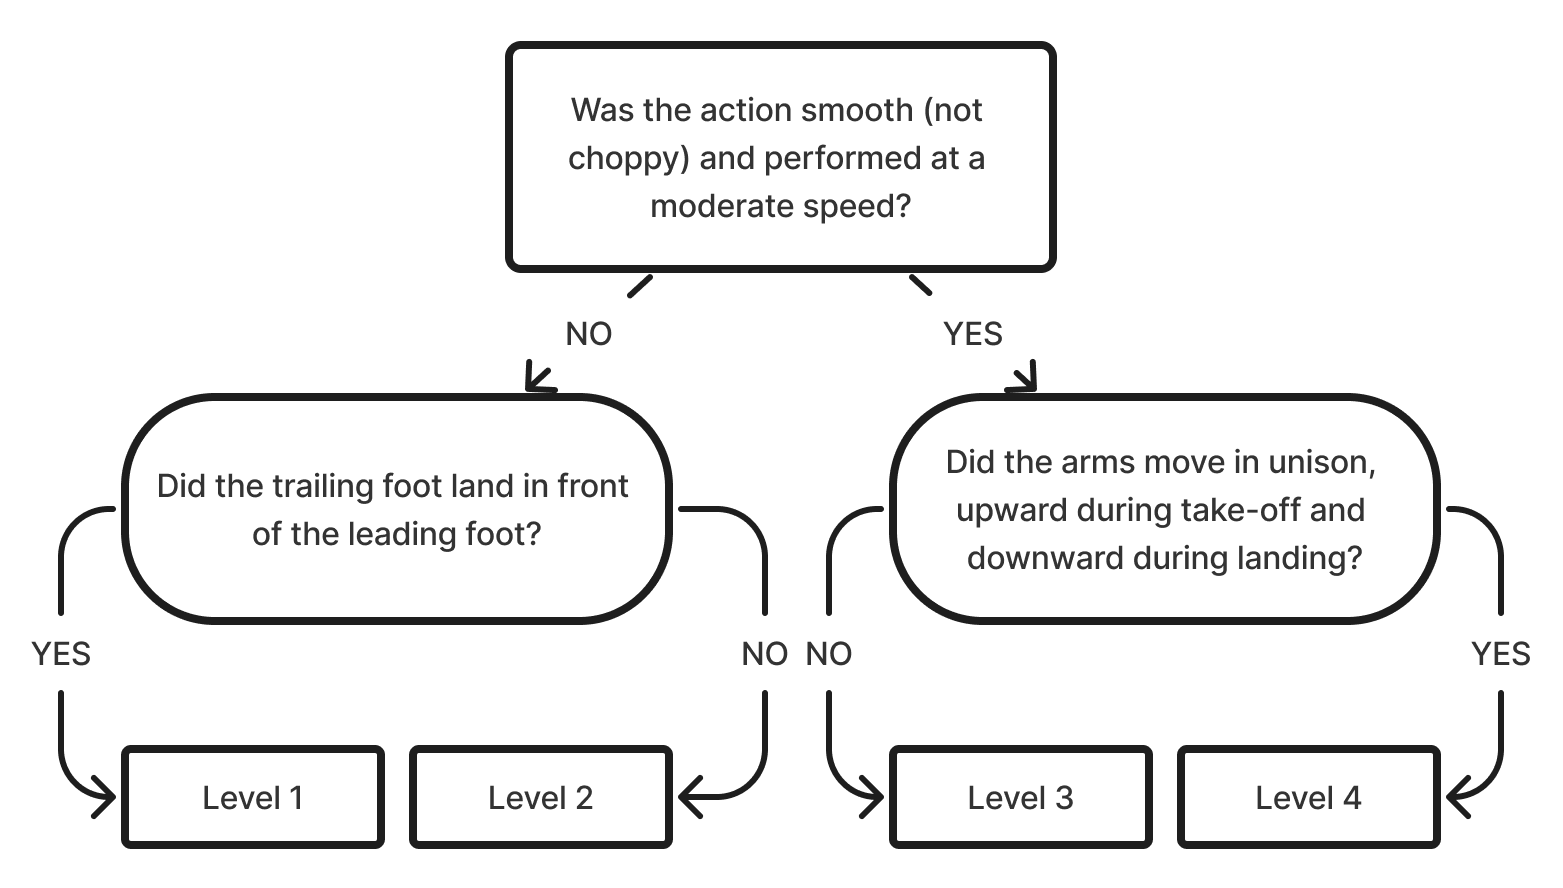
\includegraphics[keepaspectratio]{static/images/loc-gallop/scale-loc-gallop.png}}

}

\caption{\label{fig-scale-gallop}Scale for Gallop}

\end{figure}%

\subsection{Developmental Sequences}\label{developmental-sequences-9}

\begin{longtable}[]{@{}
  >{\raggedright\arraybackslash}p{(\linewidth - 2\tabcolsep) * \real{0.3500}}
  >{\raggedright\arraybackslash}p{(\linewidth - 2\tabcolsep) * \real{0.6500}}@{}}
\toprule\noalign{}
\begin{minipage}[b]{\linewidth}\raggedright
Image
\end{minipage} & \begin{minipage}[b]{\linewidth}\raggedright
Description
\end{minipage} \\
\midrule\noalign{}
\endhead
\bottomrule\noalign{}
\endlastfoot
\pandocbounded{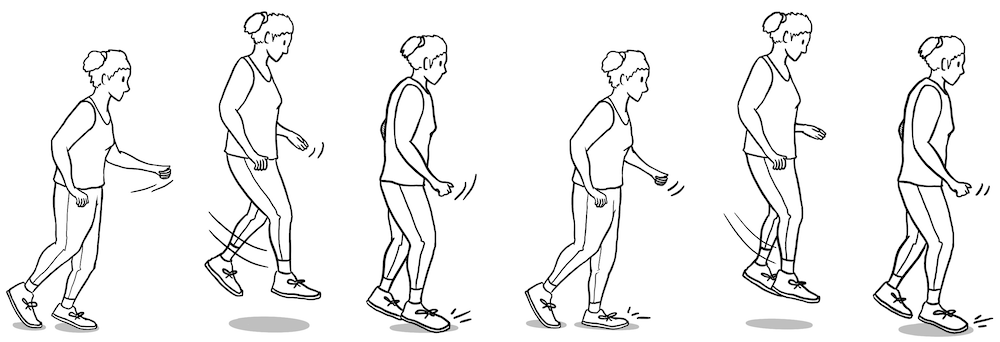
\includegraphics[keepaspectratio]{static/images/loc-gallop/ga1.png}}
& \textbf{Level 1}The action is not smooth and seems choppy/stiff. It is
often done at a fast tempo, and the trailing foot (the foot that
follows) lands in front of the leading foot. \\
\pandocbounded{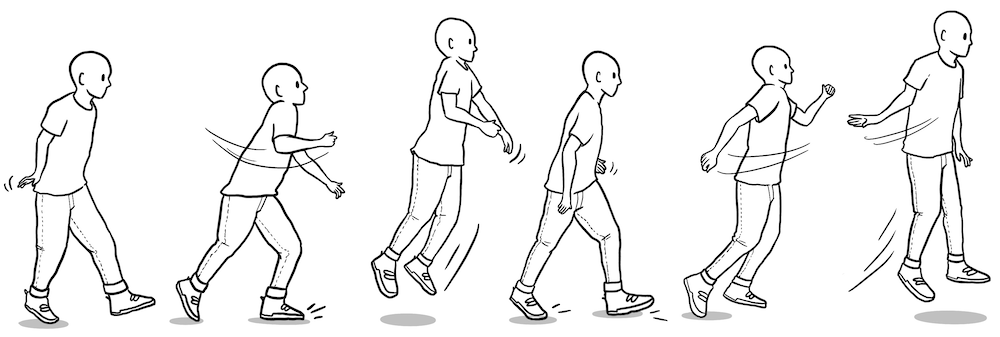
\includegraphics[keepaspectratio]{static/images/loc-gallop/ga2.png}}
& \textbf{Level 2}Still not a smooth action, but while the trailing foot
may cross the leading foot during airborne action, it does not land in
front of the leading foot. \\
\pandocbounded{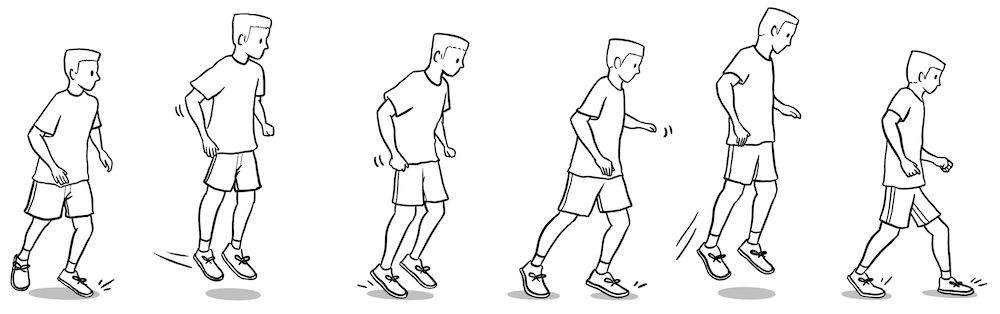
\includegraphics[keepaspectratio]{static/images/loc-gallop/ga3.png}}
& \textbf{Level 3}The action is smooth, rhythmical, and done at a
moderate tempo, but the arm action lacks a defined pattern. \\
\pandocbounded{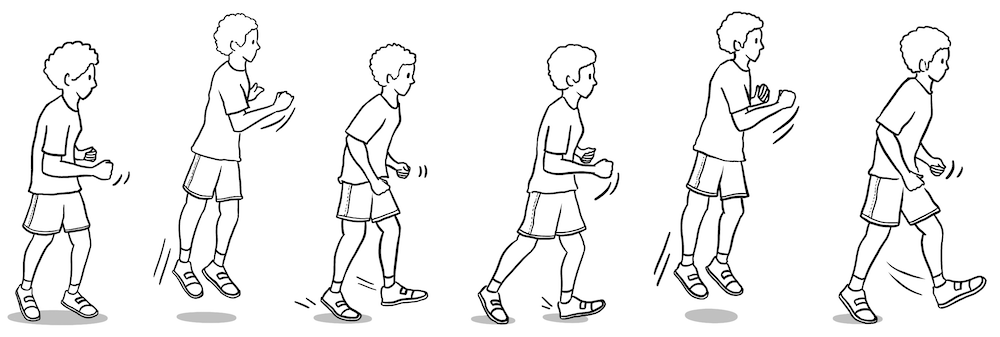
\includegraphics[keepaspectratio]{static/images/loc-gallop/ga4.png}}
& \textbf{Level 4}The action is smooth, rhythmical, and done at a
moderate speed; the arms (elbows) are lifted to waist Level at takeoff
and moved down at landing. \\
\end{longtable}

\bookmarksetup{startatroot}

\chapter*{References}\label{references}
\addcontentsline{toc}{chapter}{References}

\markboth{References}{References}

\phantomsection\label{refs}
\begin{CSLReferences}{1}{0}
\bibitem[\citeproctext]{ref-balakrishnan2023}
Balakrishnan, P., \& Ramalingam, V. (2023). The correlations between
sensory processing abilities and gross motor skills among children aged
7-10 years old. \emph{International Journal of Medical and Exercise
Science}, \emph{9}(3), 1564--1579.

\bibitem[\citeproctext]{ref-barnett2016}
Barnett, L. M., Lai, S. K., Veldman, S. L. C., Hardy, L. L., Cliff, D.
P., Morgan, P. J., Zask, A., Lubans, D. R., Shultz, S. P., Ridgers, N.
D., Rush, E., Brown, H. L., \& Okely, A. D. (2016). Correlates of Gross
Motor Competence in Children and Adolescents: A Systematic Review and
Meta-Analysis. \emph{Sports Medicine}.
\url{https://doi.org/10.1007/s40279-016-0495-z}

\bibitem[\citeproctext]{ref-bedford2015}
Bedford, R., Pickles, A., \& Lord, C. (2015). Early gross motor skills
predict the subsequent development of language in children with autism
spectrum disorder. \emph{Autism Research}, \emph{9}, 993 1001.
\url{https://onlinelibrary.wiley.com/doi/pdfdirect/10.1002/aur.1587}

\bibitem[\citeproctext]{ref-capio2022}
Capio, C., Choi, C. S. Y., \& Masters, R. (2022). Association of working
memory with gross motor skills in early childhood. \emph{International
Journal of Sport and Exercise Psychology}, \emph{21}, 992 1005.

\bibitem[\citeproctext]{ref-crane2023}
Crane, J. R., Foley, J. T., \& Temple, V. A. (2023). The Influence of
Perceptions of Competence on Motor Skills and Physical Activity in
Middle Childhood: A Test of Mediation. \emph{International Journal of
Environmental Research and Public Health}, \emph{20}(9), 5648.
\url{https://doi.org/10.3390/ijerph20095648}

\bibitem[\citeproctext]{ref-dubose2018}
DuBose, K. D., Gross McMillan, A., Wood, A. P., \& Sisson, S. B. (2018).
Joint Relationship Between Physical Activity, Weight Status, and Motor
Skills in Children Aged 3 to 10 Years. \emph{Perceptual and Motor
Skills}, \emph{125}(3), 478--492.
\url{https://doi.org/10.1177/0031512518767008}

\bibitem[\citeproctext]{ref-fathirezaie2022}
Fathirezaie, Z., Matos, S., Khodadadeh, E., Clemente, F., Badicu, G.,
Silva, A., Sani, S. H. Z., \& Nahravani, S. (2022). The relationship
between executive functions and gross motor skills in rural children
aged 8{\textendash}10 years. \emph{Healthcare}, \emph{10}(4), 616.
\url{https://doi.org/10.3390/healthcare10040616}

\bibitem[\citeproctext]{ref-fu2022}
Fu, T., Zhang, D., Wang, W., Geng, H., Lv, Y., Shen, R., \& Bu, T.
(2022). Functional training focused on motor development enhances gross
motor, physical fitness, and sensory integration in
5{\textendash}6-year-old healthy chinese children. \emph{Frontiers in
Pediatrics}, \emph{10}. \url{https://doi.org/10.3389/fped.2022.936799}

\bibitem[\citeproctext]{ref-furtado2004}
Furtado, O. Jr. (2004). \emph{Furtado-gallagher movement skill
assessment: Collecting evidence for content-related validity} {[}PhD
thesis{]}. \url{https://d-scholarship.pitt.edu/10010/}

\bibitem[\citeproctext]{ref-furtado2009}
Furtado, O. Jr. (2009). \emph{Development and initial validation of the
furtado-gallagher computerized observational movement pattern assessment
system - FG-COMPASS} {[}PhD thesis{]}.
\url{https://d-scholarship.pitt.edu/8917/}

\bibitem[\citeproctext]{ref-furtado2012}
Furtado, O. Jr., \& Gallagher, J. D. (2012). The reliability of
classification decisions for the furtado-gallagher computerized
observational movement pattern assessment system - FG-COMPASS.
\emph{Research Quarterly for Exercise and Sport}, \emph{83}(3),
383--390. \url{https://doi.org/10.1080/02701367.2012.10599872}

\bibitem[\citeproctext]{ref-furtado2018}
Furtado, O. Jr., \& Gallagher, J. D. (2018). Expert-rater agreement and
inter-/intrarater reliability for the Furtado{\textendash}Gallagher
Computerized Observational Movement Pattern Assessment System.
\emph{Perceptual and Motor Skills}, \emph{125}(3), 423--437.
\url{https://doi.org/10.1177/0031512518769205}

\bibitem[\citeproctext]{ref-gallahue2002}
Gallahue, D. L., \& Ozmun, J. C. (2002). \emph{Understanding motor
development: Infants, children, adolescents, adults}. McGraw-Hill.

\bibitem[\citeproctext]{ref-geertsen2016}
Geertsen, S. S., Thomas, R., Larsen, M. N., Dahn, I. M., Andersen, J.
N., Krause-Jensen, M., Korup, V., Nielsen, C. M., Wienecke, J., Ritz,
C., Krustrup, P., \& Lundbye-Jensen, J. (2016). Motor skills and
exercise capacity are associated with objective measures of cognitive
functions and academic performance in preadolescent children. \emph{PLoS
ONE}, \emph{11}(8), e0161960.
\url{https://doi.org/10.1371/journal.pone.0161960}

\bibitem[\citeproctext]{ref-giuriato2022}
Giuriato, M., Lovecchio, N., Pellino, V. C., Mieszkowski, J.,
Kawczyński, A., Nevill, A., \& Biino, V. (2022). Gross motor
coordination and their relationship with body mass and physical activity
level during growth in Children aged 8{\textendash}11 years old: a
longitudinal and allometric approach. \emph{PeerJ}, \emph{10}, e13483.
\url{https://doi.org/10.7717/peerj.13483}

\bibitem[\citeproctext]{ref-haywood2019}
Haywood, K. M., \& Getchell, N. (2019). \emph{Life span motor
development} (Seventh edition). Human Kinetics.

\bibitem[\citeproctext]{ref-ma2023}
Ma, F.-F., \& Luo, D.-M. (2023). Relationships between physical
activity, fundamental motor skills, and body mass index in preschool
children. \emph{Frontiers in Public Health}, \emph{11}.
\url{https://doi.org/10.3389/fpubh.2023.1094168}

\bibitem[\citeproctext]{ref-mcclenaghan1978}
McClenaghan, B. A., \& Gallahue, D. L. (1978). \emph{Fundamental
movement: Observation and assessment}. W. B. Saunders.

\bibitem[\citeproctext]{ref-perez2024}
Perez, L. (2024). Investigating Expert-Rater Agreement and
Inter/Intra-Rater Reliability of Two Fundamental Movement Skills for the
Locomotor Subscale of the FG-COMPASS. \emph{Perceptual and Motor
Skills}. \url{https://doi.org/10.1177/00315125241272720}

\bibitem[\citeproctext]{ref-peyre2019}
Peyre, H., Albaret, J.-M., Bernard, J. Y., Hoertel, N., Melchior, M.,
Forhan, A., Taine, M., Heude, B., De Agostini, M., Galéra, C., Ramus,
F., Annesi-Maesano, I., Bernard, J. Y., Botton, J., Charles, M. A.,
Dargent-Molina, P., Lauzon-Guillain, B. de, Ducimetière, P., De
Agostini, M., \ldots{} Thiebaugeorges, O. (2019). Developmental
trajectories of motor skills during the preschool period. \emph{European
Child \& Adolescent Psychiatry}, \emph{28}(11), 1461--1474.
\url{https://doi.org/10.1007/s00787-019-01311-x}

\bibitem[\citeproctext]{ref-redondo-tebar2021}
Redondo-Tebar, A., Fatouros, I. G., Martinez-Vizcaino, V., Ruíz-Hermosa,
A., Notario-Pacheco, B., \& Sanchez-Lopez, M. (2021). Association
between gross motor competence and health-related quality of life in
(pre)schoolchildren: the mediating role of cardiorespiratory fitness.
\emph{Physical Education and Sport Pedagogy}.
\url{https://www.tandfonline.com/doi/abs/10.1080/17408989.2020.1800618}

\bibitem[\citeproctext]{ref-salaj2022}
Šalaj, S., \& Masnjak, M. (2022). Correlation of motor competence and
social-emotional wellbeing in preschool children. \emph{Frontiers in
Psychology}, \emph{13}. \url{https://doi.org/10.3389/fpsyg.2022.846520}

\bibitem[\citeproctext]{ref-ulrich2000}
Ulrich, D. (2000). \emph{Test of gross motor development: {Examiner}'s
manual}. Pro-Ed.

\bibitem[\citeproctext]{ref-veldman2019}
Veldman, S. L. C., Santos, R., Jones, R. A., SousaSá, E., \& Okely, A.
(2019). Associations between gross motor skills and cognitive
development in toddlers. \emph{Early Human Development}, \emph{132},
3944.

\bibitem[\citeproctext]{ref-viegas2021}
Viegas, Â. A., Mendonça, V., Nobre, J. N. P., Morais, R. L. D. S.,
Fernandes, A. C., Ferreira, F. D. O., Figueiredo, P. H. S., Leite, H.,
Camargos, A. C. R., \& Lacerda, A. C. R. (2021). Associations of
physical activity and cognitive function with gross motor skills in
preschoolers: Cross-sectional study. \emph{Journal of Motor Behavior},
\emph{55}, 564 579.

\bibitem[\citeproctext]{ref-woolever2016}
Woolever, M. (2016). \emph{Comparing the results of the {Test} of {Gross
Motor Development-2} ({TGMD-2}) to the results of the {Furtado-Gallagher
Computerized Observational Movement Pattern Assessment System}
({FG-COMPASS})} {[}Thesis{]}. California State University, Northridge.

\bibitem[\citeproctext]{ref-zhang2023}
Zhang, L., Yao, X., Wang, Q., \& Wang, M. (2023). Gross motor skills and
development of emotional understanding of children aged 3{\textendash}6
years: Executive function as a mediator. \emph{Social Behavior and
Personality: An International Journal}.

\bibitem[\citeproctext]{ref-zuccarini2020}
Zuccarini, M., Guarini, A., Savini, S., Faldella, G., \& Sansavini, A.
(2020). Do 6-month motor skills have cascading effects on 12-month motor
and cognitive development in extremely preterm and full-term infants?
\emph{Frontiers in Psychology}, \emph{11}.
\url{https://doi.org/10.3389/fpsyg.2020.01297}

\end{CSLReferences}

\cleardoublepage
\phantomsection
\addcontentsline{toc}{part}{Appendices}
\appendix

\chapter{Appendix A: Protocols}\label{appendix-a-protocols}

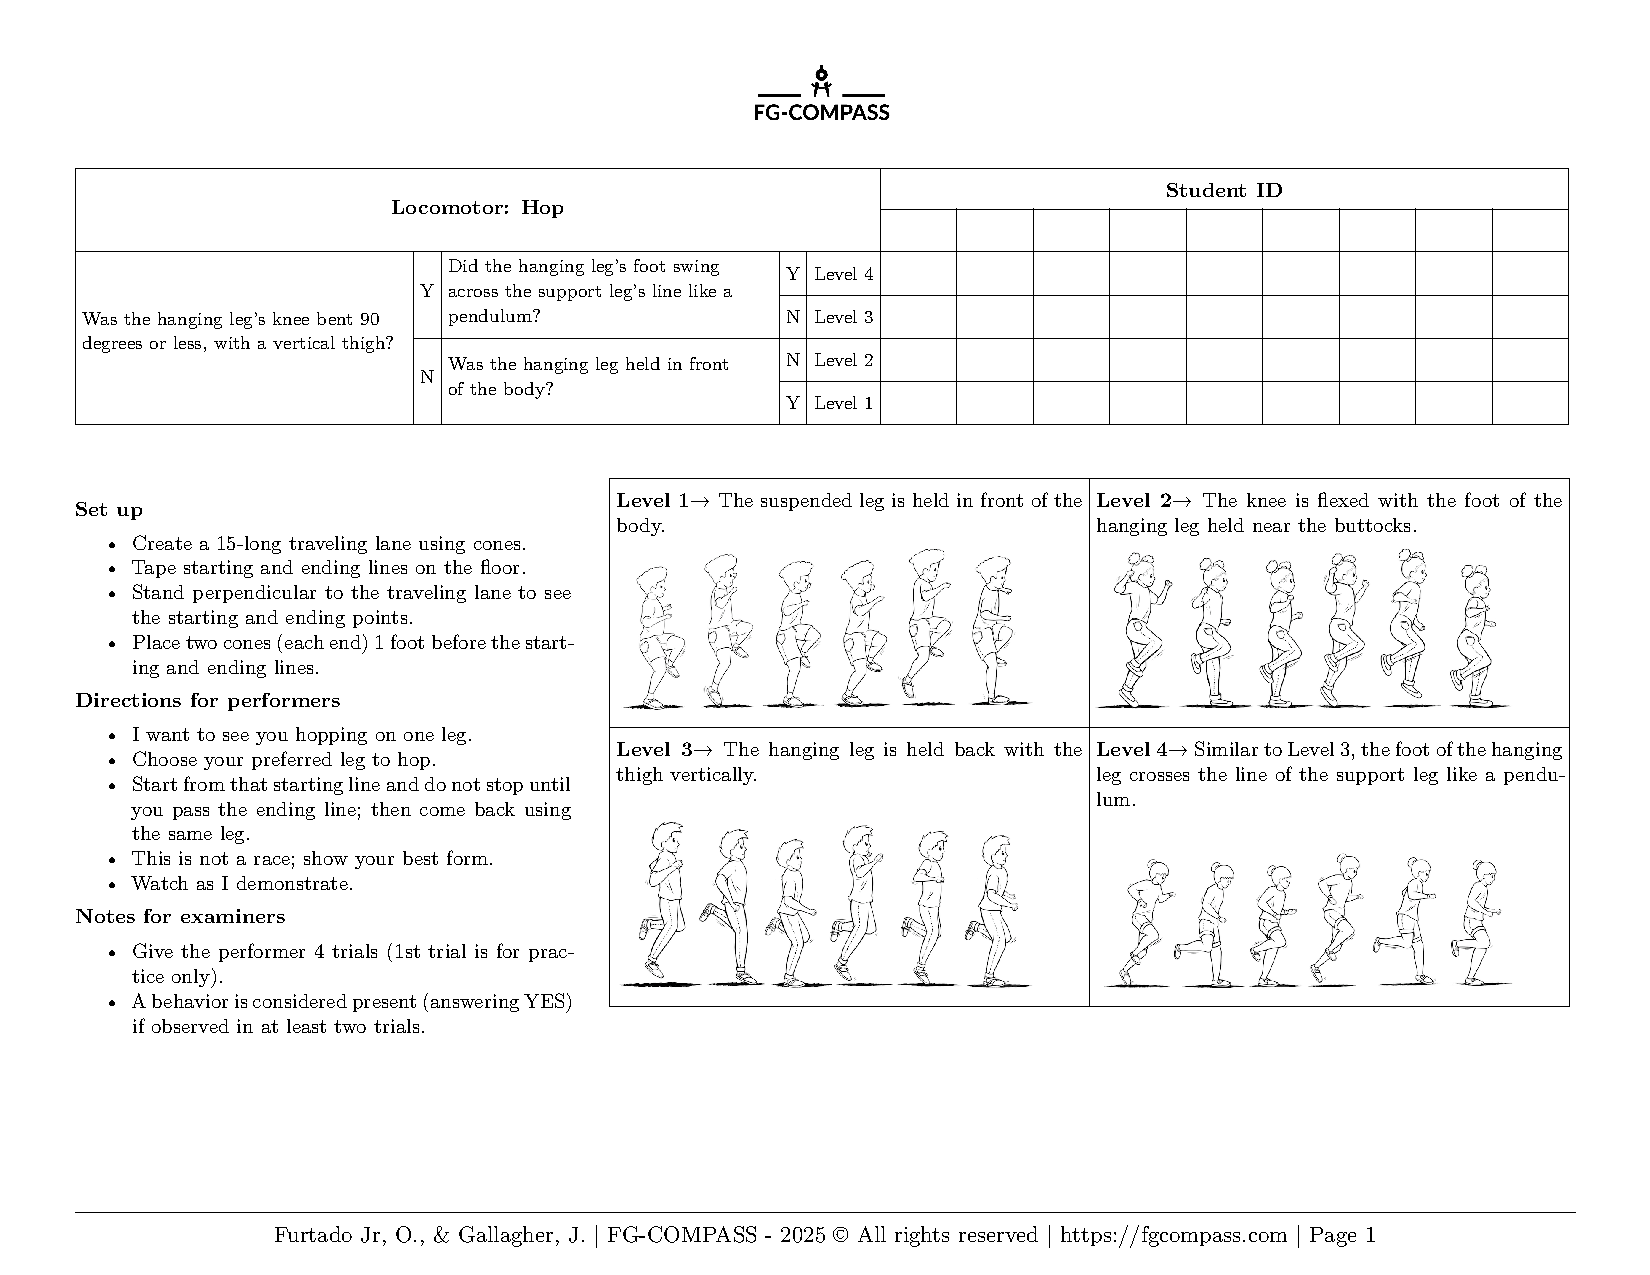
\includepdf[pages=-]{appendix-a.pdf}




\end{document}
